\documentclass{../industrial-development}
\graphicspath{{11-IT-specialist's-way/}}

\title{ Лекция №\,11 по теме «Путь специалиста в ИТ---индустрии»}
\author{ПИ---21МО Шогина Мария}
\date{2017 }


\begin{document}

\begin{frame}
  \titlepage
\end{frame}

\section{Варианты трудоустройства }

\subsection{}

\begin{frame} \frametitle{Варианты трудоустройства}
  \begin{block}{}
  Существует множество способов выгодно применять ваши навыки разработчика ПО 
  \end{block}

  \bigskip
Особо стоит отметить 3 варианта трудоустройства, такие как:
  
  \begin{itemize}
  \item Служащий
  \item Независимый консультант
  \item Предприниматель
  \end{itemize}
\end{frame}

\lecturenotes

Текст~\cite[с.~62--67]{Sonmez} со слайда

\begin{frame} \frametitle{Варианты трудоустройства: служащий}
  \begin{block}{}
    Выбор места работы, который делает большинство разработчиков ПО 
  \end{block}
  
\begin{table}[H]
\caption{\label{tab:canonsummary} Плюсы и минусы работы по найму}
\begin{center}
\begin{tabular}{|l|l|}
\hline
\textbf{Плюсы} & \textbf{Минусы} \\
\hline
Стабильность &  Недостаток свободы \\
\hline
Простейший путь  & Ограниченный доход \\
\hline
Оплаченный отпуск & \\
\hline
Помощь с медицинской страховкой & \\
\hline
\end{tabular}
\end{center}
\end{table} 

\end{frame}

\lecturenotes

Стандартный~\cite[с.~62--67]{Sonmez} и очевидный выбор места работы, который делает большинство разработчиков ПО. 
Самый большой плюс — стабильность. Под стабильностью подразумевается, что у вас постоянный источник зарабатывания денег. Если вы выбрали быть служащим, то до тех пор, пока у вас есть работа, у вас будет зарплата. В будущем есть вероятность  потерять эту работу и придется искать новую, но пока у вас период относительной стабильности, когда можно рассчитывать на определенный доход каждый месяц.

Вариант «быть служащим» также является самым простым из доступных, поскольку ваша ответственность будет ограниченна, а путь — довольно очевиден. Процесс поиска работы и трудоустройства хорошо поставлен. Вам не придется определять, что же нужно сделать, чтобы вам заплатили. У вас также будет оплачиваемый отпуск и — по крайней мере в Соединенных Штатах — помощь с медицинской страховкой.

Негативная сторона работы по найму затрагивает вашу свободу. Как служащий, вы должны тратить большую часть времени на то, чтобы решать задачи для вашего работодателя. Вы практически никак не можете повлиять на то, какую работу нужно делать, и не всегда будете делать то, что нравится. Скорее всего, также придется соблюдать расписание: сколько часов в неделю вы должны работать.

Несмотря на то что ваш доход известен заранее, он, скорее всего, будет иметь верхнюю границу. Будучи служащим, вы в конце концов достигнете потолка доходов и возможностей продвижения по карьерной лестнице.


\begin{frame} \frametitle{Варианты трудоустройства: независимый консультант}
  \begin{block}{}
    Независимый консультант --- это разработчик ПО, который не работает на конкретного работодателя 
  \end{block}
  
   \begin{table}[H]
\caption{\label{tab:canonsummary} Плюсы и минусы работы независимым консультантом }
\begin{center}
\begin{tabular}{|p{0.5\linewidth}|p{0.5\linewidth}|}
\hline
\textbf{Плюсы} & \textbf{Минусы} \\
\hline
Больше свободы &  Приходится искать клиентов \\
\hline
Постоянно появляются новые проекты  & Нагрузка, связанная с ведением бизнеса \\
\hline
Возможность зарабатывать больше денег & Несколько начальников вместо одного \\
\hline
\end{tabular}
\end{center}
\end{table} 
\end{frame}

\lecturenotes

Многие~\cite[с.~62--67]{Sonmez} разработчики ПО зарабатывают на жизнь независимыми консультантами. Независимый консультант — это разработчик ПО, который не работает на конкретного работодателя. Вместо этого у него один или несколько клиентов. Если у вас когда-нибудь была работа на стороне, когда вы программировали для клиента, который оплачивал труд по часам (или сумма была заранее оговоренной), вы знаете, что значит быть консультантом.
Разработчик считается независимым консультантом, если он получает большую часть своего дохода подобным образом.

 Консультант отличается от разработчика ПО, работающего по контракту, поскольку последний трудится только на одного  клиента. Работа по контракту ближе к работе по найму. Независимый консультант обычно имеет собственную компанию, которая заключает контракты на выполнение работ, но при этом он не привязан к одному клиенту.
Нельзя сказать, что профессия независимого консультанта имеет сплошные минусы. В том, что вы отчитываетесь не одному работодателю, есть и плюсы. Как независимый консультант вы можете самостоятельно определять рабочие часы, а также работу, за которую будете браться. Вы можете приходить и уходить в любое время и составлять гибкое расписание, но клиенты будут ожидать от вас того, что работа будет выполнена своевременно.

Самый большой плюс — это, скорее всего, потенциальный заработок. Как независимый консультант вы можете получать в час гораздо больше, чем работая на кого-то. 

Несмотря на то что может показаться, что работа независимым консультантом приносит немалый доход, много времени уходит на поиск клиентов и прочие задачи, связанные с управлением бизнесом. Если вы независимый консультант, то фактически являетесь бизнесом (не только в ваших мыслях). Вы отвечаете за уплату налогов, юридические вопросы, продажи, здоровье и все остальное, что связано с ведением бизнеса.


\begin{frame} \frametitle{Варианты трудоустройства: предприниматель}
  \begin{block}{}
 Путь предпринимателя самый трудный, самый неопределенный и потенциально самый прибыльный
  \end{block}
  
  \begin{table}[H]
\caption{\label{tab:canonsummary} Плюсы и минусы предпринимательской деятельности }
\begin{center}
\begin{tabular}{|p{0.5\linewidth}|p{0.5\linewidth}|}
\hline
\textbf{Плюсы} & \textbf{Минусы} \\
\hline
Полная свобода &  Высокие риски \\
\hline
Потенциально высокий заработок  & Можно рассчитывать только на себя \\
\hline
Работаете над тем, что нравится & Требуется владеть множеством других навыков \\
\hline
Нет начальника  & Придется много работать \\
\hline
\end{tabular}
\end{center}
\end{table} 

\end{frame}

\lecturenotes

Путь~\cite[с.~62--67]{Sonmez} предпринимателя, возможно, самый трудный, самый неопределенный и потенциально самый прибыльный. Этому есть объяснение. Этот вариант не несет никакой стабильности, но если вам повезет, то по-крупному.

Определение этого пути довольно расплывчатое и может значить множество разных вещей. Разработчика считается предпринимателем, если он развивает свой бизнес или продукт с использованием профессиональных навыков. В то время как служащий и независимый консультант меняют свое время на деньги, предприниматель меняет свое время не на моментальную выручку, а на шанс получить высокую оплату в будущем.

Разработчики-предприниматели создают стартапы и ищут финансирование у внешних инвесторов, которое называется венчурным капиталом. Или открывают маленькие компании, работающие по принципу «программа как служба» (software-as-a-service, SaaS), и зарабатывают деньги, продавая подписки на их службу. Например, основатели популярной службы по обучению разработчиков Pluralsight начали с обучения людей в кабинетах. Но позднее поняли, что могут улучшить качество услуг, перенеся обучение в Интернет, поэтому перешли к модели SaaS и начали предлагать службу, основанную на подписке.

Я уверен, что вы теперь самостоятельно можете определить два самых больших преимущества предпринимательской деятельности: полная свобода и неограниченные возможности заработка. У вас не будет начальника, кроме самого. Вы можете приходить на работу и уходить когда вздумается, вы полностью отвечаете за свое будущее. Вы также можете зарабатывать миллионы долларов, если создадите очень успешный продукт. Кроме того, если правильно вложиться в собственное время, то ваши доходы от этого могут вырасти экспоненциально.

Но предпринимательская деятельность включает в себя риск. Доход совершенно не гарантирован, и вы можете залезть в долги, пытаясь реализовать свои гениальные идеи. Жизнь предпринимателя похожа на американские горки. В один день у вас есть покупатели — и вы чувствуете, будто находитесь на вершине мира. На следующий день о проекте забывают — и вам приходится ломать голову, как оплатить счета.

Предпринимательство также требует от вас развития навыков, о которых не нужно беспокоиться, если вы работаете на кого-то или являетесь независимым консультантом. Предприниматели должны изучить продажи, маркетинг, а также другие аспекты ведения бизнеса и финансов, которые являются важными составляющими успеха. 

%\section{}

\section{Возможные пути развития специалиста }

\subsection{2.1 Развитие  специалиста по ступеням профессионального мастерства }


\subsection{}

\begin{frame} \frametitle{Развитие  специалиста по ступеням профессионального мастерства}
  \begin{block}{}
  По мере того как вы приобретаете более соответствующий опыт работы, вы можете постепенно занимать более высокие позиции
 \end{block}
\bigskip
Выделяют 4 основных позиции:
  
  \begin{itemize}
  \item Младший(Стажер) --- Junior
  \item Старший --- Middle
  \item Ведущий --- Senior
 \item Главный --- Lead
  \end{itemize}
\end{frame}

\lecturenotes

Текст со слайда~\cite{JMSL}

Официальная градация, пропагандируемая работными сайтами~\cite{hh}, и на которую ориентируется большинство, выглядит так:
	0,5-1,5 года реального опыта = Junior

	1-3 года = Middle 

	4-6 лет = Senior

	>6 лет = Lead


\begin{frame} \frametitle{Развитие  специалиста по ступеням профессионального мастерства}
 \centerline{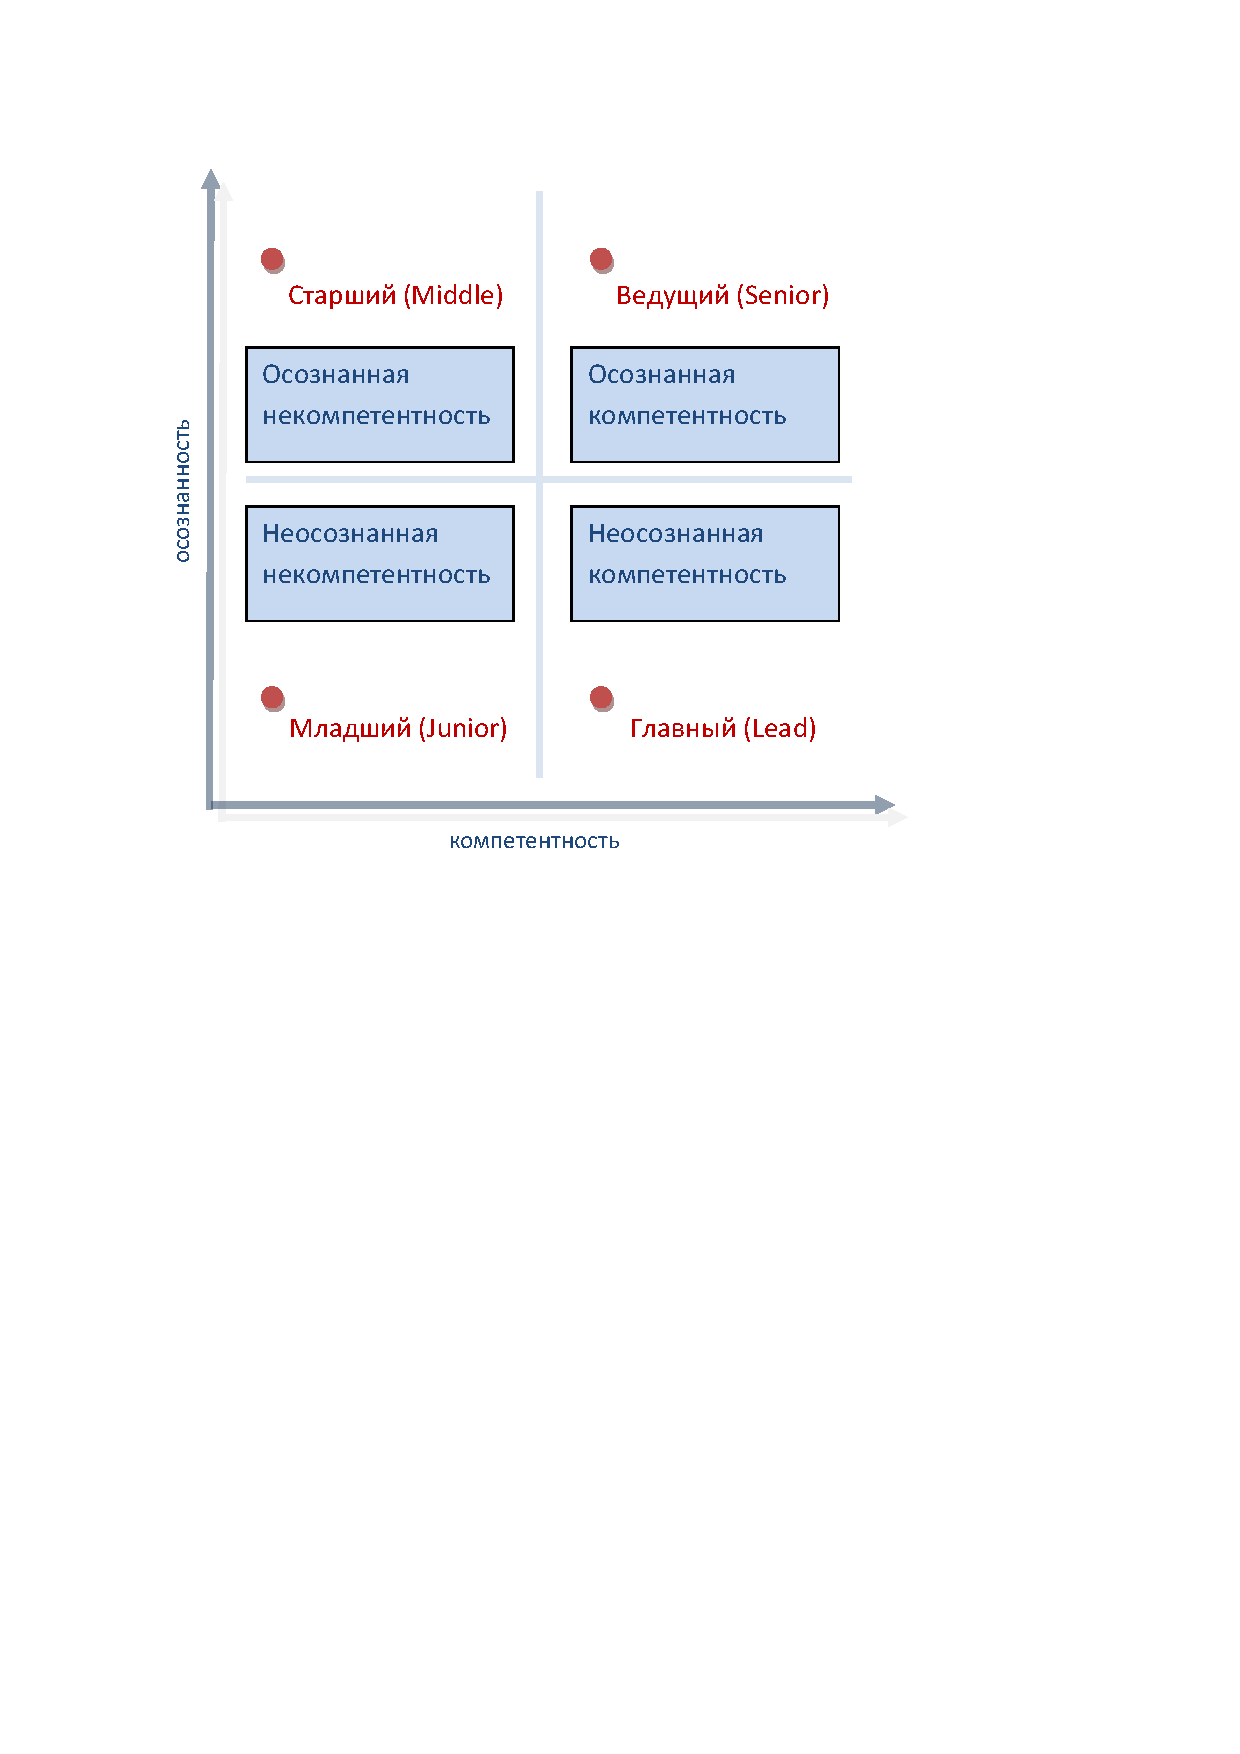
\includegraphics[width=1.05\linewidth]{11-IT-specialist's-way/11.pdf}}

\end{frame}

\lecturenotes

Junior~\cite{JMSL}

Люди на этой позици, не могут представить объем работы в той или иной области, ответственности. Многие находятся в квадрате «Неосознанная некомпетентность» по многим своим навыкам. Люди, процентное понимание области которых примерно 0 - 25%. 

Middle 

Навыки, которые были у junior на уровне 0 – 25, на этом этапе перейдут в 25 – 50%. По факту: для многих навыков фокус сместится в “Осознанную некомпетентность”. Появление практической базы навыков. Таким образом, то, что знал junior на базовом уровне, middle уже знает более глубоко, но все же еще не эксперт в этой области. 

Senior

Многие вещи оказываются в квадрате «осознанная компетентность». В этом квадрате навыки, в которых вы уже реально разбираетесь и умеете применить на практике, а также можете объяснить другим. Человек выступает как консультант по этим навыкам, у него многогранный опыт в этой области.

Lead

По факту: для многих навыков фокус сместится в “Неосознанную компетентность”.Lead это Senior к обязанностям которого добавляются еще и обязанности по управлению командой, формирования стратегий развития, контролю исполнения бизнес-процессов. Контролирует работу нижестоящего персонала, обучает новичков.


%\section{}

\subsection{2.2 Развитие  специалиста в иерархии компании  }

\subsection{}

\begin{frame} \frametitle{Развитие  специалиста в иерархии компании: полная схема }
  \centerline{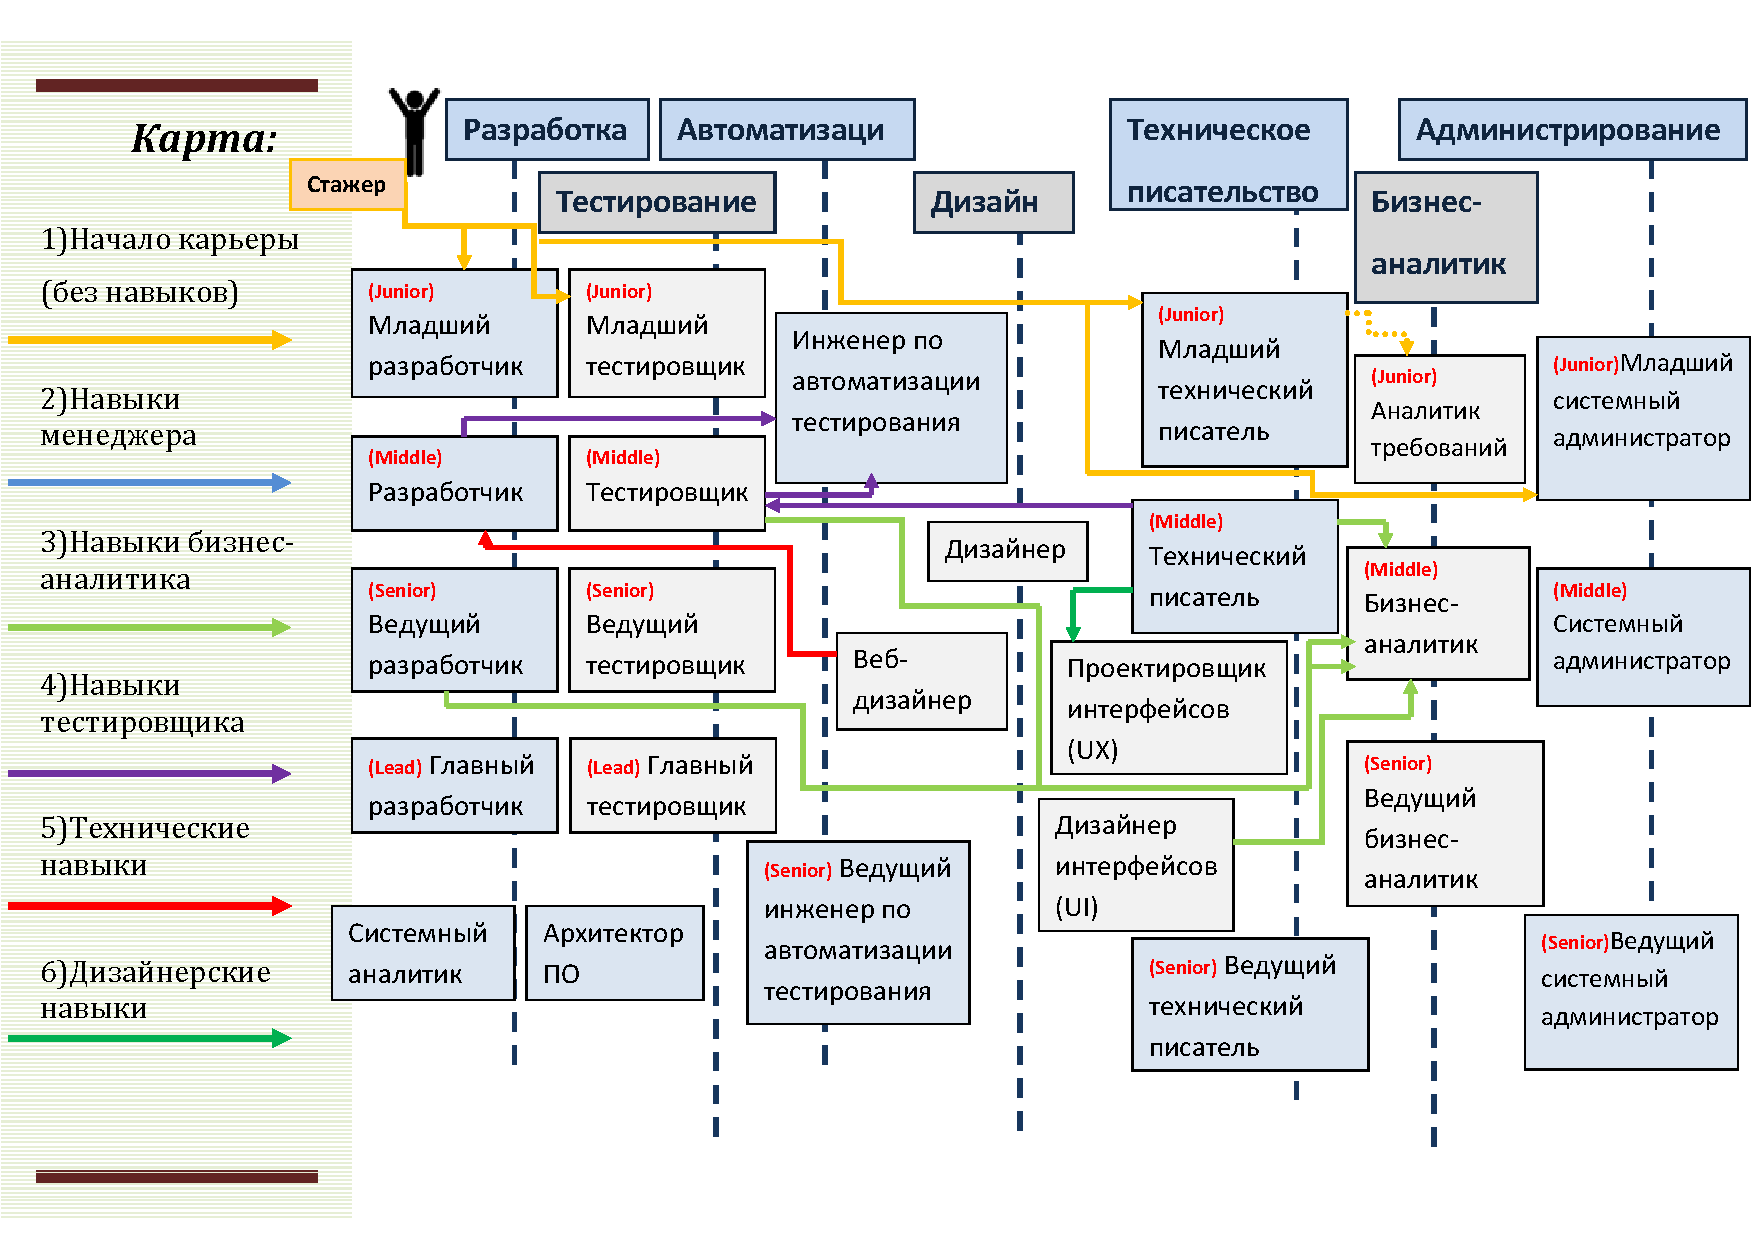
\includegraphics[height=0.92\textheight]{11-IT-specialist's-way/schNew11.pdf}}
\end{frame}

\lecturenotes

Развитие  специалиста по ступеням профессионального мастерства ,безусловно важно, так как влечет за собой и развитие специалиста в иерархии компании.

Так~\cite{mc} выглядит полная схема развития специалиста в иерархии компании.Анализ схемы начнется с позиции- стажера. Также  будут рассмотрены вертикальные и косвенные переходы между различными специальностями внутри ит рынка. Карта схемы поможет более быстро и легко разбираться в косвенных переходах.Имеет смысл рассматривать данную схему более подробно по частям.

\begin{frame} \frametitle{Развитие  специалиста в иерархии компании: 1 часть из 4 }
  \centerline{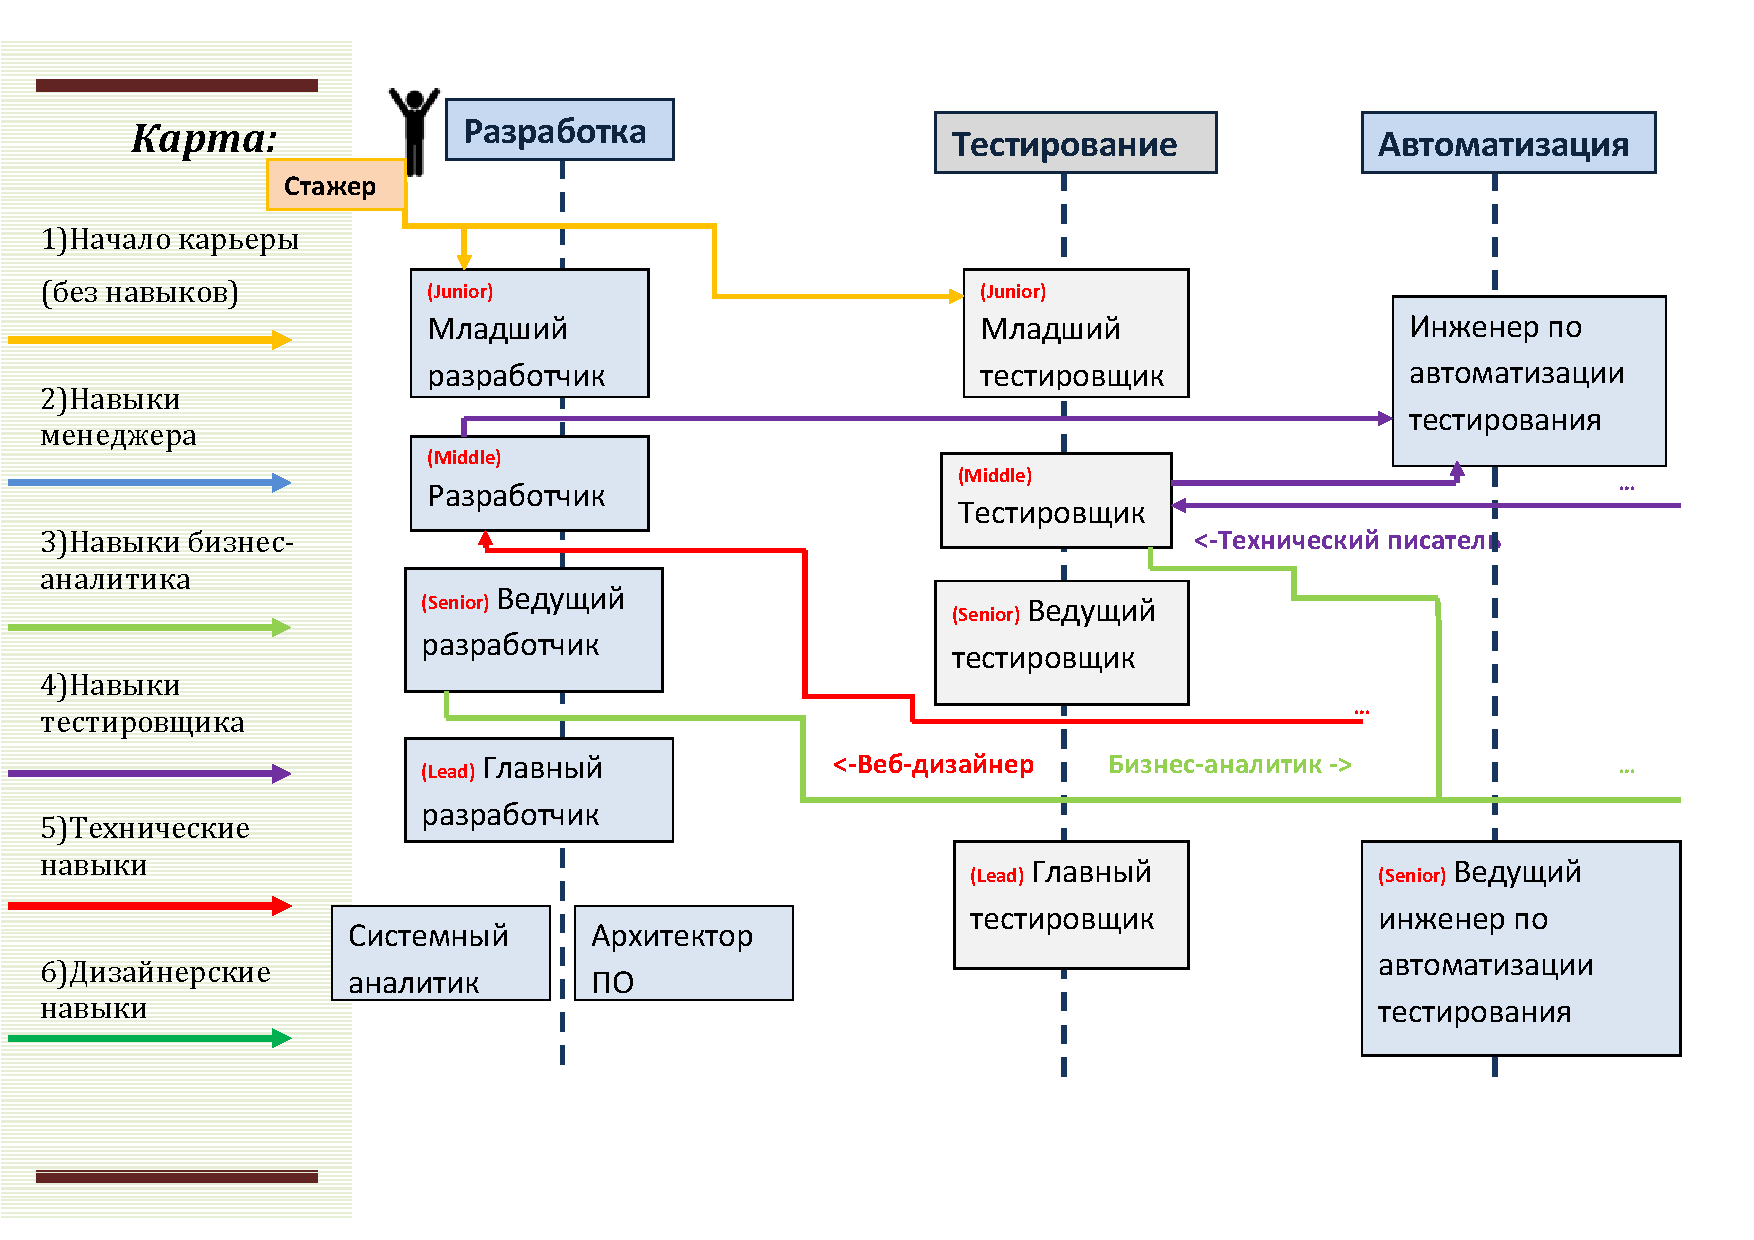
\includegraphics[width=1.14\linewidth]{11-IT-specialist's-way/schNew2.pdf}}
\end{frame}

\lecturenotes

В 1 части оказались 3 сегмента ит рынка, такие как: Разработка,Тестирование, Автоматизация.

Прмые переходы:

1) 1ым прямым переходом --- является переход внутри сегмента, связанного с разработкой

2) 2ым прямым переходом --- является переход внутри сегмента, связанного с тестированием

3) 3им прямымпереходом --- является переход внутри сегмента, связанного с автоматизацией


\begin{frame} \frametitle{ Развитие разработчика внутри специальности}
 \centerline{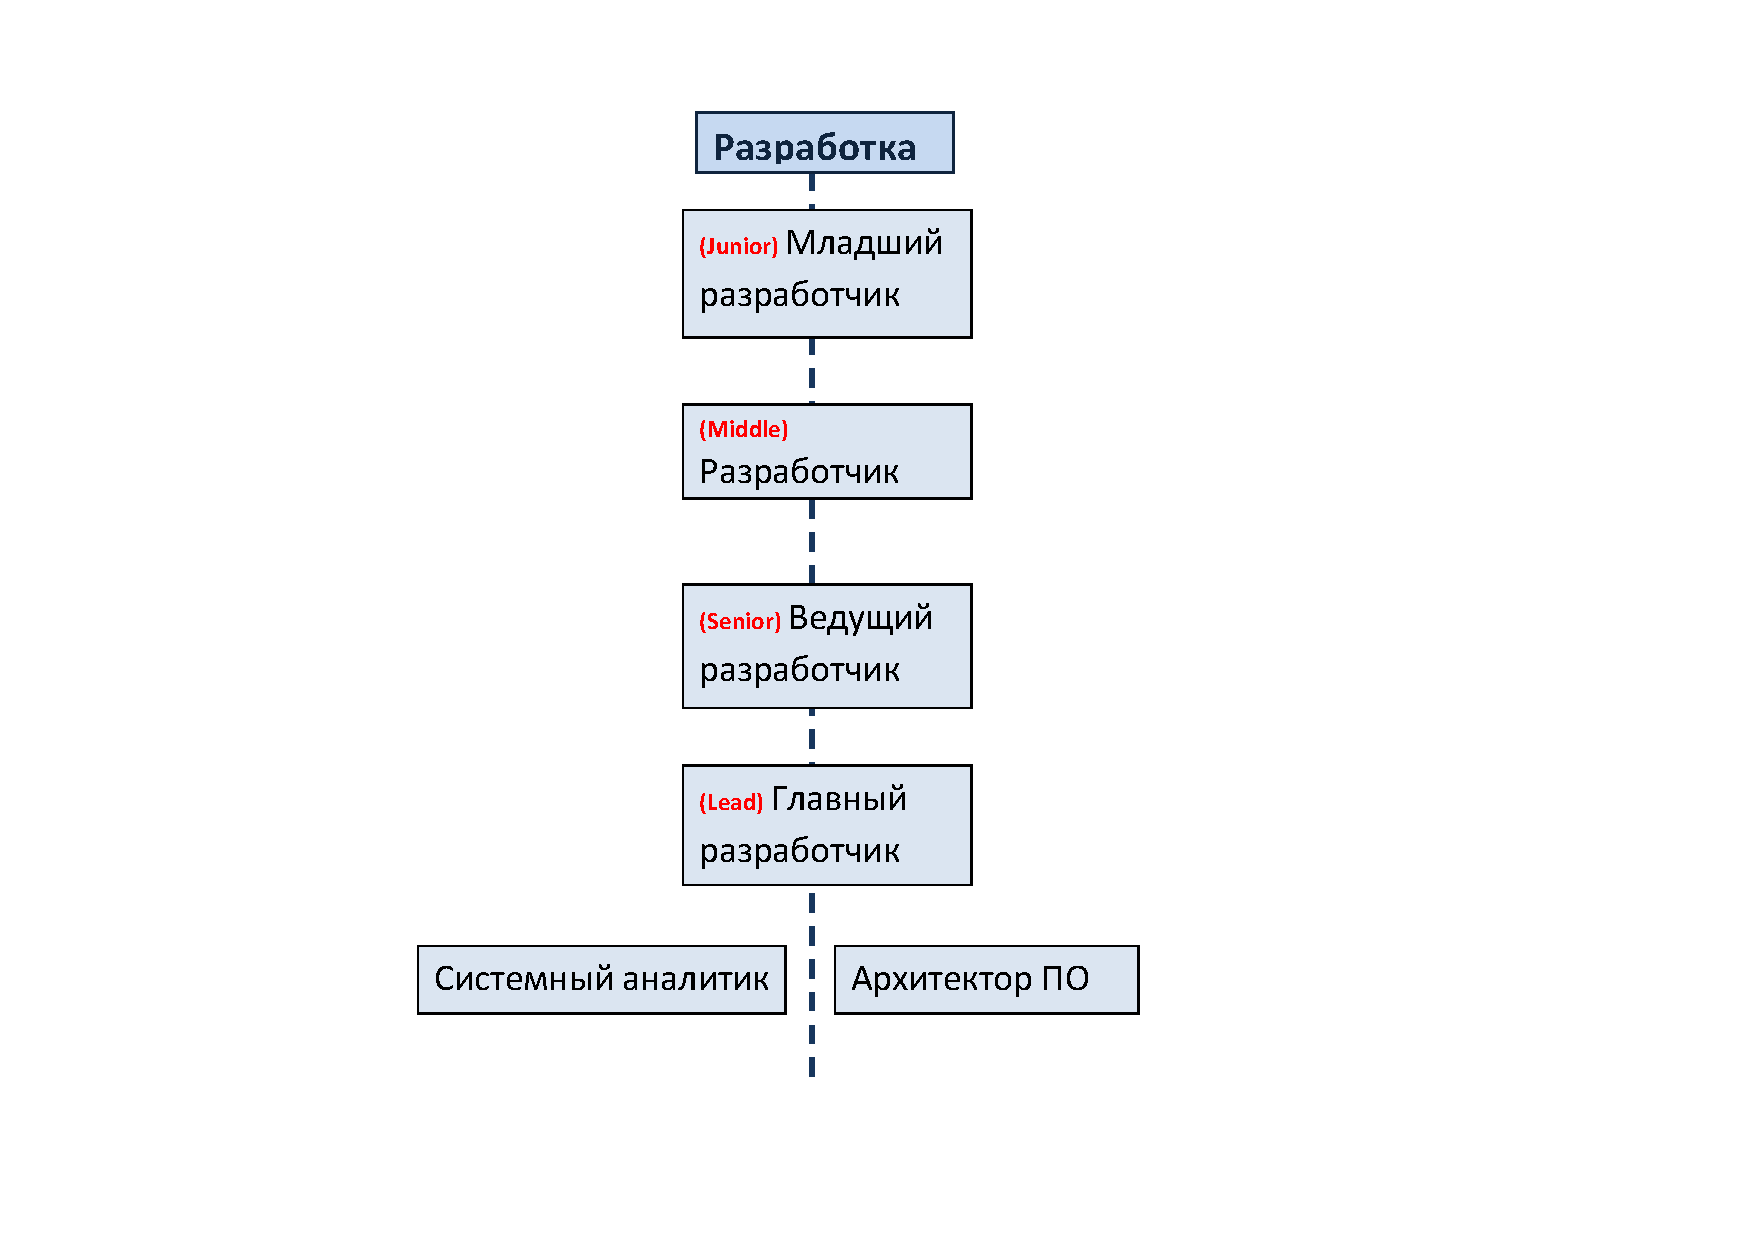
\includegraphics[width=1.18\linewidth]{11-IT-specialist's-way/schNew6.pdf}}
\end{frame}

\lecturenotes
 
1ым~\cite{mc} прямым переходом --- является переход внутри сегмента, связанного с разработкой. Далее рассмотрим подробнее

\begin{frame} \frametitle{Развитие разработчика внутри специальности: младший разработчик}
 \begin{block}{}
  \alert{Позиция --- младший разработчик (Junior Developer)}

Должностные обязанности: 
  \end{block}
  \begin{itemize}
  \item Сопровождение существующих корпоративных программ и приложений
  \item Переработка архитектуры приложения (уменьшение сцепленности компонент для обеспечения расширяемости и надёжности, внедрение многопоточности для повышения скорости работы 

и отзывчивости приложения, вынесение части логики в независимые скрипты для увеличения гибкости)
  \item Создание объектов в БД
  \end{itemize}
\end{frame}

\lecturenotes

Позиция – Младший~\cite{itcf} разработчик~\cite{hh}

Должностные обязанности~\cite{rab}:

Сопровождение существующего корпоративного портала.

Переработка архитектуры приложения (уменьшение сцепленности компонент для обеспечения расширяемости и надёжности, внедрение многопоточности для повышения скорости работы и отзывчивости приложения, вынесение части логики в независимые скрипты для увеличения гибкости)

 
Создание объектов в БД.


\begin{frame} \frametitle{Развитие разработчика внутри специальности: разработчик}
 \begin{block}{}
  \alert{Позиция --- разработчик (Middle Developer)}

Должностные обязанности в отличие от младшего разработчика: 
  \end{block}
  \begin{itemize}
  \item Решение задач по интеграции кода программного продукта
  \item Умение организовать  команду, обучение кадров
  \item Рефакторинг кода
  \end{itemize}
\end{frame}

\lecturenotes

Позиция~\cite{hh} – Разработчик ~\cite{itcf}

Должностные обязанности~\cite{rab}:

Решение задач по интеграции кода программного продукта;

Сопровождение и документирование кода;

Умение организовать  команду, обучение кадров;

 Рефакторинг кода


\begin{frame} \frametitle{Развитие разработчика внутри специальности: ведущий разработчик}
 \begin{block}{}
  \alert{Позиция --- ведущий разработчик (Senior Developer)}

Должностные обязанности в отличие от разработчика: 
  \end{block}
  \begin{itemize}
  \item Разработка модификаций информационной системы
  \item Проведение первичного тестирования разработанных модификаций информационной системы
 \item  Участие в автоматизации тестирования 

и развертывания
  \item Обеспечение контроля безопасности создаваемых продуктов на всех этапах
  \end{itemize}
\end{frame}

\lecturenotes

Позиция – Ведущий~\cite{hh} разработчик~\cite{itcf}

Должностные обязанности~\cite{rab} :

• Разработка модификаций  информационной системы;

• Проведение первичного тестирования разработанных модификаций;

• Участие в автоматизации тестирования и развертывания;

• Обеспечение контроля безопасности создаваемых продуктов на всех этапах;

\begin{frame} \frametitle{Развитие разработчика внутри специальности: главный разработчик}
 \begin{block}{}
  \alert{Позиция --- главный разработчик (Lead Developer)}

Должностные обязанности в отличие от ведущего разработчика: 
  \end{block}
  \begin{itemize}
  \item Оценка изменений системного кода
  \item Коммуникации с командами архитекторов, аналитиков и тестировщиков
 \item  Отчетность перед руководством о ходе разработки
  \end{itemize}
\end{frame}

\lecturenotes

Позиция – Главный~\cite{hh} разработчик~\cite{itcf}

Должностные обязанности~\cite{rab}:

Оценка изменений системного кода;

Коммуникации с командами архитекторов, аналитиков и тестировщиков;

Отчетность перед руководством о ходе разработки; 

\begin{frame} \frametitle{Развитие разработчика внутри специальности: системный аналитик}
 \begin{block}{}
  \alert{Позиция --- системный аналитик (Systems Analyst)}

Должностные обязанности в отличие от разработчика: 
  \end{block}
  \begin{itemize}
\item  Изучает и систематизирует документацию по проекту, выделяет процессы, подлежащих автоматизации
  \itemГотовит документацию по описанию сущностей, взаимосвязей и процессов предметной области 

с использованием специальных нотаций
  \item Собирает, анализирует и документирует функциональные требования к ПО
 \item  Анализирует риски и причины возникновения ошибок при разработке систем
 \item Выбирает платформы для реализации проекта
  \end{itemize}
\end{frame}

\lecturenotes

Позиция – Системный~\cite{hh} аналитик~\cite{itcf}

Должностные обязанности~\cite{rab}:

•	Изучает ту или иную область на предмет внедрения и/или разработки прикладных информационных систем. 

•	Участвует в интервьюировании (совместно с бизнес-аналитиками) бизнес-экспертов и пользователей информационных систем на предмет изучения текущих принципов организации хода процессов (в том числе с точки зрения функционирования информационных систем). 

•	Изучает и систематизирует документацию по проекту в части выделения процессов, подлежащих автоматизации. 

•	Готовит документацию по описанию сущностей, взаимосвязей и процессов предметной области с использованием специальных нотаций. 

•	Участвует в постановке задач и разработке технического задания. 

•	Собирает, анализирует и документирует функциональные требования к программному обеспечению. 

•	Подготавливает схемы тестирования функционала для выявления отклонений от сформулированных бизнес-требований и функциональных требований. 

•	Тестирует прототип разрабатываемой системы. 

•	 Обучает пользователей системы. 

•	Анализирует риски и причины возникновения ошибок при разработке систем. 

•	Выбирает платформы для реализации проекта. 

\begin{frame} \frametitle{Развитие разработчика внутри специальности: архитектор ПО}
 \begin{block}{}
  \alert{Позиция --- архитектор ПО (Software Architect)}

Должностные обязанности в отличие от разработчика: 
  \end{block}
  \begin{itemize}
\item  Разработка ТЗ, проектов, обоснований с точки зрения экономики, разработка концепций и стратегий, программы реализации проекта
  \item Разработка методологии для адаптации системы

 к той структуре, которая есть в организации
  \item Подготовка и ведение отчетности по архитектуре, контроль соблюдения архитектурных решений
 \item Анализ качества установленного ПО и соответствия его необходимым требованиям
  \end{itemize}
\end{frame}

\lecturenotes

Позиция – Архитектор~\cite{hh} ПО~\cite{itcf}
Должностные обязанности~\cite{rab}: 

•	Проектирование баз данных, информационных систем, ПО. 

•	Разработка ТЗ, проектов, обоснований с точки зрения экономики. Разработка концепций и стратегий, а также программы реализации. 

•	Разработка архитектуры ПО, алгоритма, согласно которому оно будет работать, технологии и способа обработки информации. 

•	Разработка методологии для адаптации системы к той структуре, которая есть в организации. 

•	Координация проекта по вопросам взаимодействия между исполнителями (группы аналитиков, заказчиком, техподдержкой, информационной безопасностью). 

•	Надзор, а также руководство процессом выполнения проекта. 

•	Осуществление процесса контроля по вопросам внедрения разработанных решений, новых систем, а также приложений. 

•	Предоставление консультаций пользователям проекта. 

•	Подготовка и ведение отчетности по архитектуре. Контроль соблюдения архитектурных решений.

•	 Контроль соответствия разработки решению. 

•	Координация планирования.

•	 Разработка архитектуры систем. 

•	Анализ качества установленного ПО и соответствия его необходимым требованиям. 


\begin{frame} \frametitle{Развитие тестировщика внутри специальности }
  \centerline{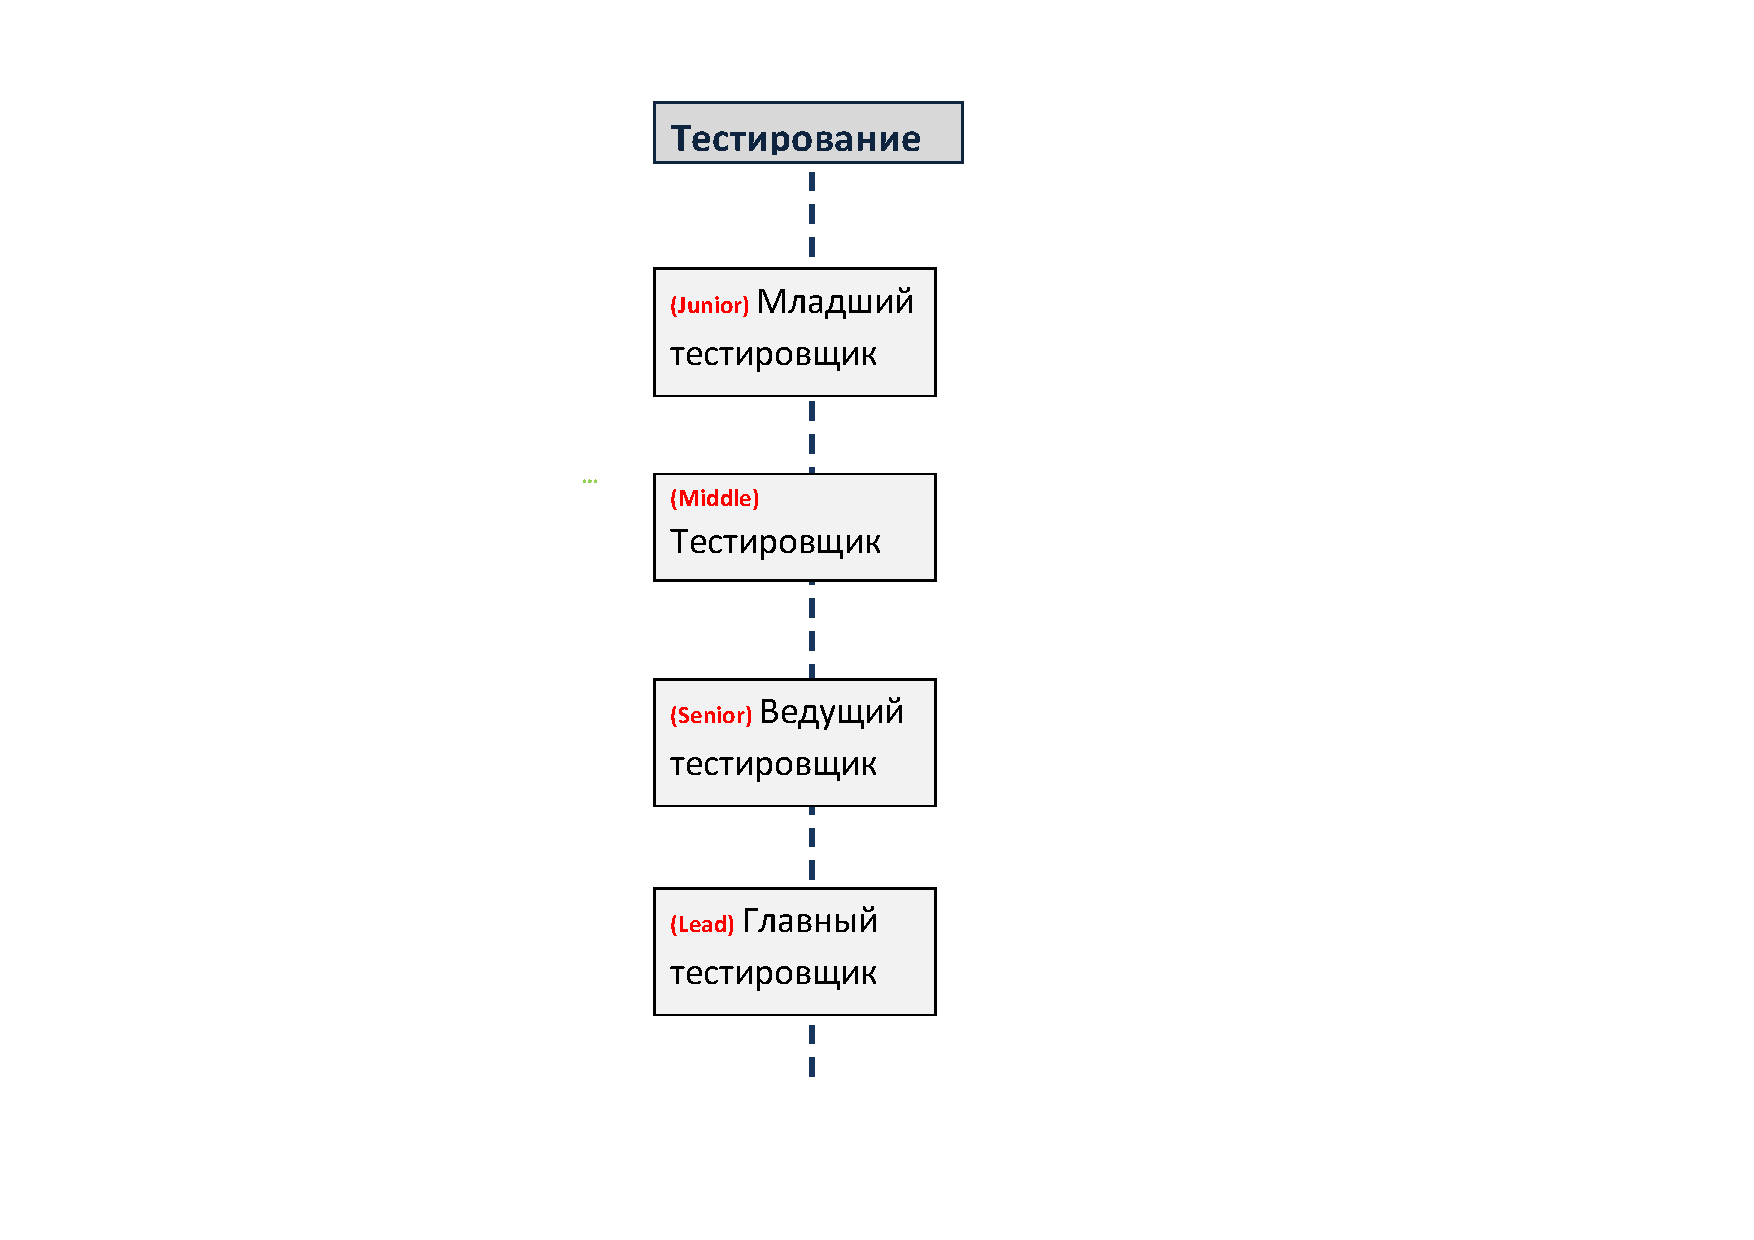
\includegraphics[width=1.19\linewidth]{11-IT-specialist's-way/schNew7.pdf}}
\end{frame}
\lecturenotes

 2ым~\cite{mc} прямым переходом  - является переход внутри сегмента, связанного с тестированием. Далее рассмотрим подробнее


\begin{frame} \frametitle{Развитие тестировщика внутри специальности: младший тестировщик}
 \begin{block}{}
  \alert{Позиция --- младший тестировщик (Junior QA)}

Должностные обязанности: 
  \end{block}
  \begin{itemize}
  \item Проведение ручного тестирования разделов приложения
  \item Создание и поддержка тест-кейсов
  \item Взаимодействие с другими подразделениями компании для организации эффективной работы
 \item Общение с ИТ-службами для разбора найденных ошибок
\item Документальное сопровождение деятельности
  \end{itemize}
\end{frame}

\lecturenotes

Позиция – Младший~\cite{hh} тестировщик~\cite{itcf}
Должностные обязанности~\cite{rab}: 

•	проведение ручного тестирования разделов приложения;

•	создание и поддержка тест-кейсов;

•	Взаимодействие с другими подразделениями компании для организации эффективной работы.

•	Общение с ИТ-службами для разбора найденных ошибок.

•	Документальное сопровождение деятельности.

\begin{frame} \frametitle{Развитие тестировщика внутри специальности: тестировщик}
 \begin{block}{}
  \alert{Позиция --- тестировщик (Middle QA)}

Должностные обязанности в отличие от младшего тестировщика: 
  \end{block}
  \begin{itemize}
  \item Проведение функционального и регрессивного тестирования, cоставление отчетов по итогам проведенного тестирования
  \item Анализ требований и ТЗ на предмет корректности
  \item Работа в системе баг-трекинга
  \end{itemize}
\end{frame}

\lecturenotes

Позиция – Тестировщик~\cite{hh} QA~\cite{itcf}
Обязанности~\cite{rab}:

•	проведение функционального и регрессивного тестирования, cоставление отчетов по итогам проведенного тестирования;

•	анализ требований и ТЗ на предмет корректности;

•	работа в системе баг-трекинга.

\begin{frame} \frametitle{Развитие тестировщика внутри специальности: ведущий тестировщик}
 \begin{block}{}
  \alert{Позиция --- ведущий тестировщик (Senior QA)}

Должностные обязанности в отличие от тестировщика: 
  \end{block}
  \begin{itemize}
  \item Постоянное взаимодействие с командой разработки
  \item Уточнение требований к ПО заказчика 

или бизнес-аналитиков
  \item Оценка возможных рисков
 \item Внедрение идей оптимизации рабочего процесса
 \item Обучение кадров
  \end{itemize}
\end{frame}

\lecturenotes

Позиция – Ведущий~\cite{hh} тестировщик~\cite{itcf}

ЗАДАЧИ~\cite{rab}:
•	постоянное взаимодействие с командой разработки;

•	уточнение требований к ПО заказчика или бизнес-аналитиков;

•	оценка возможных рисков;

•	внедрение идей оптимизации рабочего процесса.

•	обучение кадров.


\begin{frame} \frametitle{Развитие тестировщика внутри специальности: главный тестировщик}
 \begin{block}{}
  \alert{Позиция --- главный тестировщик (Lead QA)}

Должностные обязанности в отличие от ведущего тестировщика: 
  \end{block}
  \begin{itemize}
  \item Руководство работами по созданию тестовых спецификаций, подготовке к тестированию, проведению тестирования, составлению и обработке отчетов
  \item Отчетность перед менеджером проекта и начальником отдела о ходе выполнения поставленных задач
  \item Оценка возможных рисков
 \item Планировать работы по автоматизации тестирования
  \end{itemize}
\end{frame}

\lecturenotes

Позиция – Lead QA~\cite{hh} (Главный тестировщик)~\cite{itcf}
Обязанности~\cite{rab}:

•	Руководство работами по созданию тестовых спецификаций, подготовке к тестированию, проведению тестирования, составлению и обработке отчетов.

•	Отчетность перед менеджером проекта и/или начальником отдела о ходе выполнения поставленных задач.

•	Планировать работы по автоматизации тестирования;




\begin{frame} \frametitle{Развитие инженера по автоматизации тестирования внутри специальности: }
  \centerline{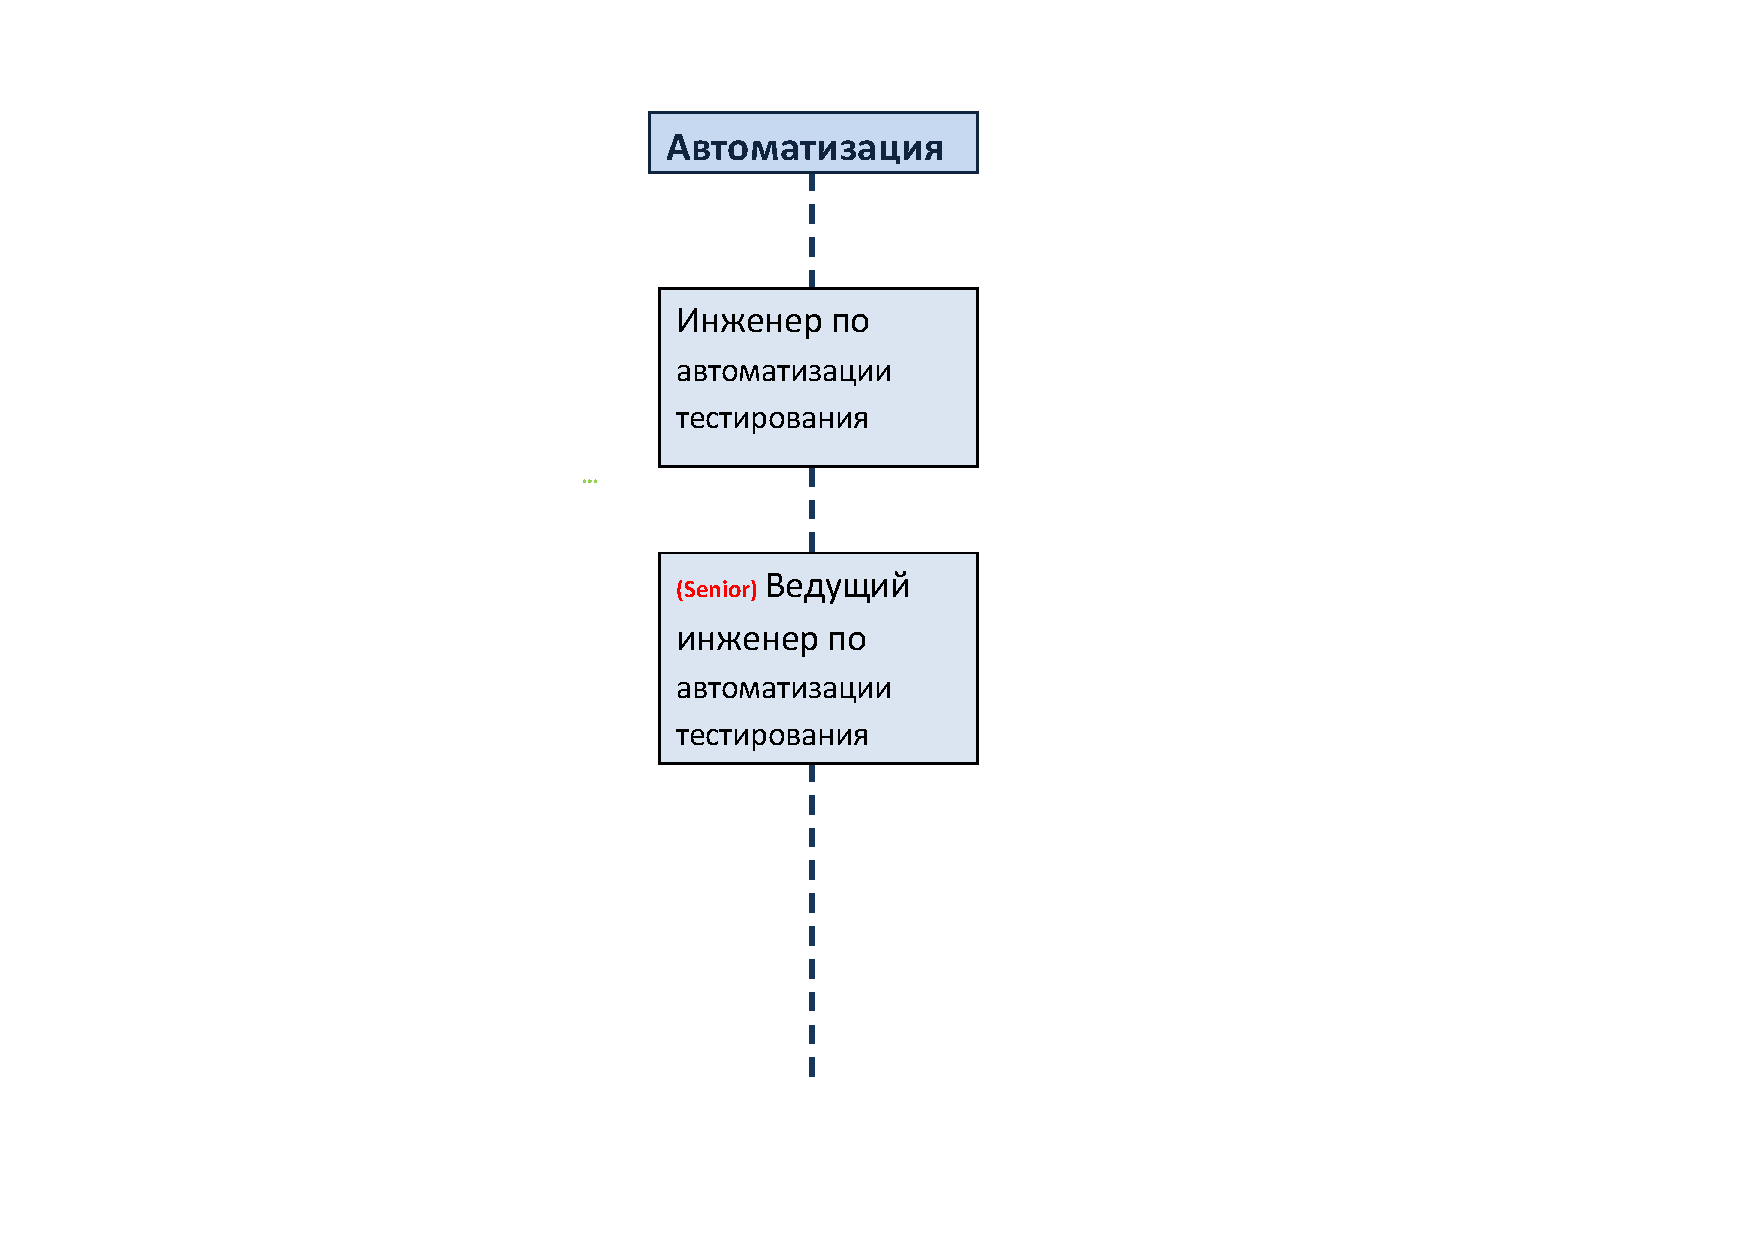
\includegraphics[width=1.15\linewidth]{11-IT-specialist's-way/schNew8.pdf}}
\end{frame}

\lecturenotes

 3ей~\cite{mc} прямой веткой  - является ветка внутри сегмента, связанного с автоматизацией. Далее рассмотрим подробнее

\begin{frame} \frametitle{Развитие инженера по автоматизации тестирования внутри специальности: инженер по автоматизации тестирования }
 \begin{block}{}
  \alert{Позиция ---  инженер по автоматизации тестирования (Middle Automatization QA)}

Должностные обязанности в отличие от тестировщика: 
  \end{block}
  \begin{itemize}
  \item Разработка и поддержка специализированного фреймворка для автоматизированного тестирования
  \item  Разработка тестов для функциональности устройства по низкоуровневой документации 
  \item Поддержка и запуск тестов в рамках системы автоматического автоматизированного тестирования, коммуникация с другими группами по результатам тестирования
  \end{itemize}
\end{frame}

\lecturenotes

Позиция – инженер по автоматизации~\cite{hh} тестирования~\cite{itcf}
Задачи~\cite{rab}:

- Разработка и поддержка специализированного фрэймворка для автоматизированного тестирования.

- Разработка тестов для определенной функциональности устройства по низкоуровневой документации на устройство.

- Поддержка и запуск тестов в рамках системы автоматического автоматизированного тестирования и коммуникация с другими группами (в рамках и за пределами команды) в зависимости от результатов тестирования.

- Визуализация результатов тестирования и ее последующая автоматизация.

\begin{frame} \frametitle{Развитие инженера по автоматизации тестирования внутри специальности: ведущий инженер по автоматизации тестирования }
 \begin{block}{}
  \alert{Позиция --- ведущий инженер по автоматизации тестирования (Senior Automatization QA)}

Должностные обязанности в отличие от мнженера 

по автоматизации тестирования: 
  \end{block}
  \begin{itemize}
  \item Обучение кадров
  \item  Участие в планировании направления деятельности
  \item Внедрении новых правил, методов работы 

и стандартов тестирования
 \item Координирование основной деятельности 

с внутренними отделами и внешними поставщиками
  \end{itemize}
\end{frame}

\lecturenotes

Позиция – Ведущий  инженер по автоматизации~\cite{hh} тестирования~\cite{itcf}
Задачи~\cite{rab}:

•	Обучение кадров

•	Участие в планировании деятельности направления

•	Внедрении новых правил, методов работы и стандартов тестирования

•	Координирование основной деятельности с внутренними отделами и внешними поставщиками





\begin{frame} \frametitle{Косвенные переходы между специальностями: 1 часть из 4}


Косвенные переходы представляют собой набор навыков, необходимых для перехода из одной специальности 

в другую

 \bigskip
 \begin{block}{Технические навыки}
 Развивая \alert{технические навыки}, у специалиста появляется возможность переходов: 
\begin{itemize}
  \item Разработчик ---> Инженер по автоматизации тестирования
  \item Тестировщик ---> Инженер по автоматизации тестирования
  \end{itemize}
  \end{block}
\end{frame}


\begin{frame} \frametitle{Косвенные переходы между специальностями: мотивация }

 \begin{block}{Тестировщик --->  Инженер по автоматизации тестирования  

Разработчик --->  Инженер по автоматизации тестирования }
Мотивы, обуславливающие данные переходы:
  \end{block}
\begin{itemize}
\item Познавательный мотив (стремление ~к овладеванию специальными знаниями)
\item Эстетический мотив (желание работать по данной специальности)
\item Материальный мотив (стремление иметь более высокооплачиваемую работу) 
\item Престижный мотив (стремление к работе, обеспечивающей более быстрое продвижение 

по службе)
  \end{itemize}
\end{frame}

\lecturenotes

Выявлены несколько групп мотивов выбора профессии:

1. социальные (желание своим трудом способствовать общественному прогрессу, занять достойное место в обществе в соответствии с интересами и возможностями);

2. моральные (приносить пользу людям, оказывать им помощь, общение);

3. эстетические (стремление к красоте, гармонии, желание работать по специальности, связанной с прекрасным);

4. познавательные (связанные со стремлением к овладению специальными знаниями, проникновением в сущность профессиональной деятельности);

5. творческие (возможность быть оригинальным, неповторимым);

6. материальные (стремление иметь высокооплачиваемую работу, льготы);

7. престижные (стремления, позволяющие достичь видного положения в обществе, избрание профессии, обеспечивающей быстрое продвижение по службе, профессии, которая «ценится среди друзей и знакомых»);

8. утилитарные (возможность работать в городе, иметь «чистую» работу, близко к дому, легкость поступления в вуз, на работу, советы и примеры друзей и знакомых).

 \begin{frame} \frametitle{Косвенные переходы между специальностями: возможности }

 \begin{block}{Тестировщик --->  Инженер по автоматизации тестирования    

Разработчик --->  Инженер по автоматизации тестирования }
Возможно при дополнительном изучении:
  \end{block}
\begin{itemize}
  \item Принципов разработки и поддержки специализированного фреймворка 

для автоматизированного тестирования
  \item Требований к корректному запуску тестов в рамках системы автоматического автоматизированного тестирования
\item Требований к визуализации результатов тестирования
  \end{itemize}
\end{frame}

\lecturenotes


Тестировщик --------- инженер по автоматизации~\cite{hh} тестирования~\cite{itcf}
Возможно при дополнительном умении:
•	Разработка и поддержка специализированного фрэймворка для автоматизированного тестирования.
•	Поддержка и запуск тестов в рамках системы автоматического автоматизированного тестирования и коммуникация с другими группами (в рамках и за пределами команды) в зависимости от результатов тестирования.
•	Визуализация результатов тестирования и ее последующая автоматизация.


Разработчик--------- инженер по автоматизации~\cite{hh} тестирования~\cite{itcf}
Возможно при дополнительном умении:
•	Разработка и поддержка специализированного фрэймворка для автоматизированного тестирования.
•	Поддержка и запуск тестов в рамках системы автоматического автоматизированного тестирования и коммуникация с другими группами (в рамках и за пределами команды) в зависимости от результатов тестирования.
•	Визуализация результатов тестирования и ее последующая автоматизация.


\begin{frame} \frametitle{Развитие  специалиста в иерархии компании: 2 часть из 4 }
  \centerline{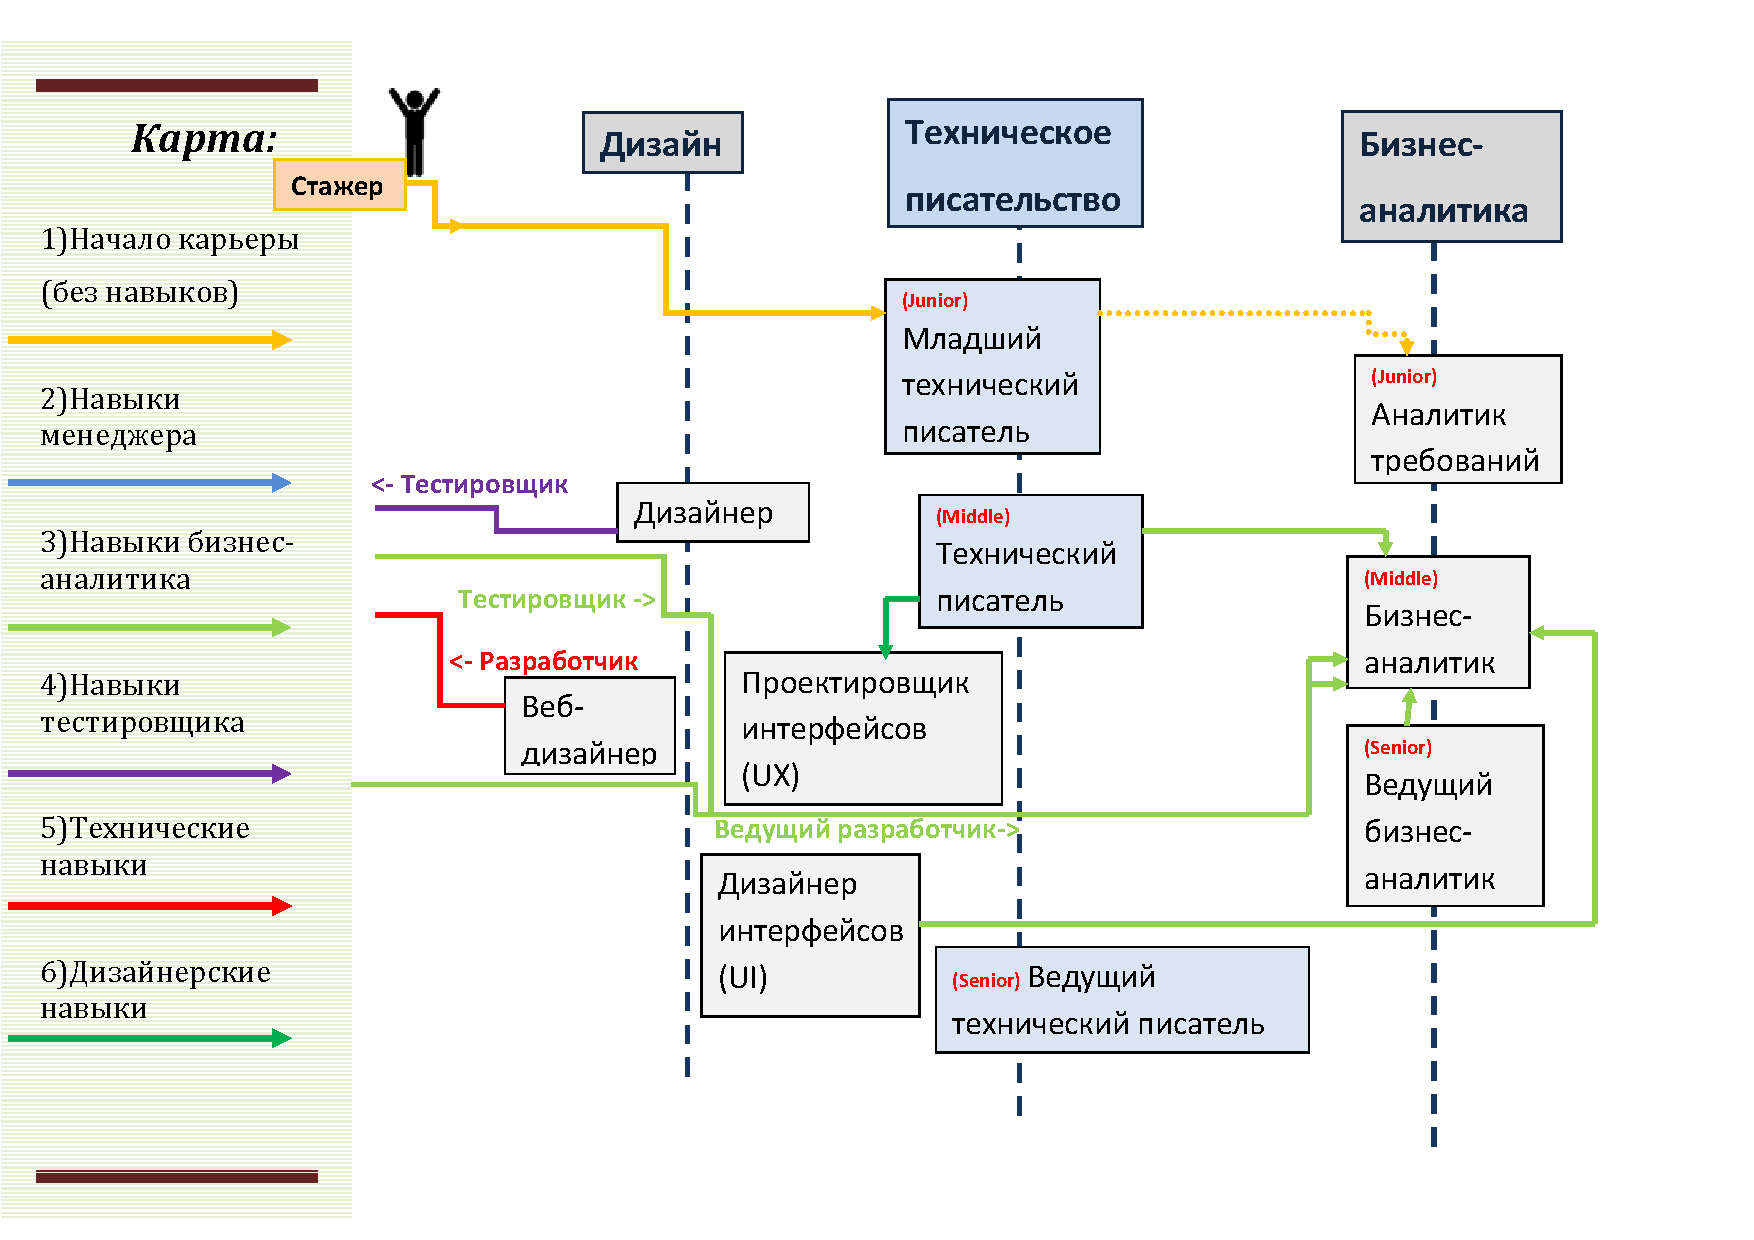
\includegraphics[width=1.125\linewidth]{11-IT-specialist's-way/schNew3.pdf}}
\end{frame}

\begin{frame} \frametitle{Развитие дизайнера внутри специальности}
  \centerline{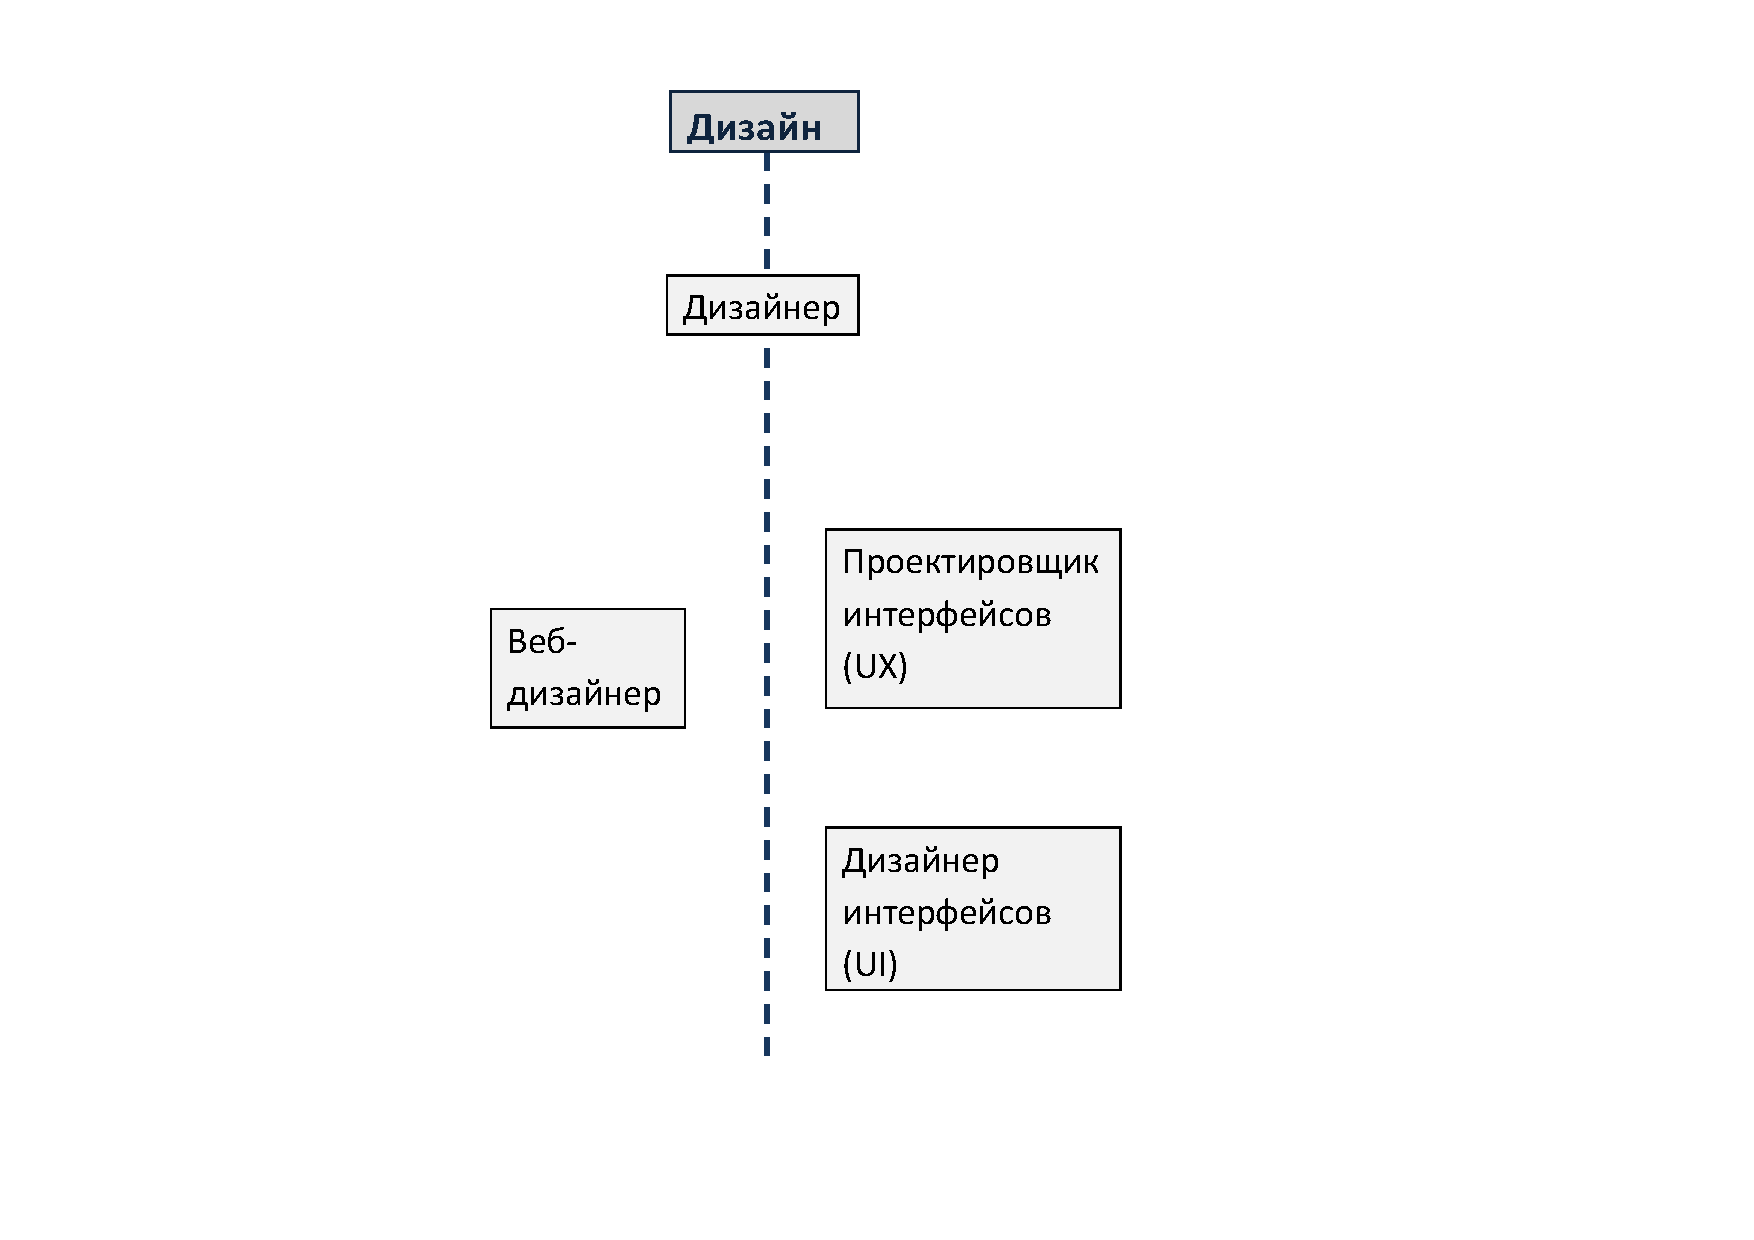
\includegraphics[width=1.19\linewidth]{11-IT-specialist's-way/schNew9.pdf}}
\end{frame}

\lecturenotes

 1ым~\cite{mc} прямым переходом  - является переход внутри сегмента, связанного с дизайном. Подробнее далее.

\begin{frame} \frametitle{Развитие дизайнера внутри специальности: дизайнер }
 \begin{block}{}
  \alert{Позиция --- дизайнер (Designer)}

Должностные обязанности: 
  \end{block}
  \begin{itemize}
  \item  Выполнение художественно-оформительских работ 

по заказам подразделений предприятия (клиентов)
  \item  Составление эскизов и согласовывание эскизов 

с непосредственным руководителем 
  \item Консультирует своего непосредственного руководителя (клиента) о принципах и вариантах решения поставленных дизайнерских задач
 \item  Вносит исправления в проекты художественного 

и технического оформления по указанию художественного редактора
  \end{itemize}
\end{frame}

\lecturenotes

Позиция~\cite{hh} – Дизайнер~\cite{itcf}
Должностные обязанности~\cite{rab}:

1.	Осуществляет своевременное и качественное выполнение художественно-оформительских работ по заказам подразделений предприятия (клиентов).

2.	Разрабатывает проекты художественного и технического оформления изданий исходя из информации, полученной от непосредственного руководителя или клиента (об адресной аудитории, о цели издания, о сроках выполнения, о требуемом качестве, пр.).

3.	Составляет эскизы и выполняет работы по художественному оформлению публикаций различного характера (в журналах, книгах, иных изданиях), проектов, отчетов, информационных и рекламных материалов; разрабатывает эскизы упаковки, товарных знаков, пр.

4.	Консультирует своего непосредственного руководителя (клиента) о принципах и вариантах решения поставленных дизайнерских задач.

5.	Согласовывает эскизы (проекты) с непосредственным руководителем (клиентом) и подготавливает окончательные макеты информационных изданий (пресс-релизов, объявлений, бюллетеней, ведомостей, прайс-листов, справочников, пр.), идентифицирующих материалов (визитных карточек, этикеток, упаковки, бланков, пр.), справочных изданий (адресных книг, учебных и иных пособий, пр.), художественно-публицистических изданий (книг, журналов, газет, пр.).

6.	Вносит исправления в проекты художественного и технического оформления по указанию художественного редактора.

\begin{frame} \frametitle{Развитие дизайнера внутри специальности: веб-дизайнер }
 \begin{block}{}
  \alert{Позиция --- веб-дизайнер (Web Designer)}

Должностные обязанности в отличие от дизайнера: 
  \end{block}
  \begin{itemize}
  \item   Разработка концепции дизайна и интерфейса web-сайта
  \item  Отрисовка дизайна макетов (технический дизайн) разделов, страниц, интерфейсов, модулей
  \item Подготовка и размещение на сайте графики и контента
 \item Оптимизация дизайна существующих и разработка новых интерфейсов
  \end{itemize}
\end{frame}

\lecturenotes

Позиция – Веб~\cite{hh} Дизайнер~\cite{itcf}
Должностные обязанности web-дизайнера~\cite{rab}:

- разработка концепции дизайна и интерфейса web-сайта;

- отрисовка дизайн-макетов (технический дизайн) разделов, страниц, интерфейсов, модулей;

- создание графических и стилистических элементов для сайтов, дизайн баннеров и промостраниц, создание презентаций;

- подготовка и размещение на сайте графики и контента;

- оптимизация дизайна существующих и разработка новых интерфейсов.

- заполнение, продвижение и поддержка работы сайта,

- макетирование и верстка полиграфической продукции для внутреннего использования (бланки, буклеты, визитки).

\begin{frame} \frametitle{Развитие дизайнера внутри специальности: дизайнер 

и проектировщик интерфейсов }
 \begin{block}{ Дизайнер интерфейсов (UI дизайнер)}
Занимается  отрисовкой интерфейса на основе UX данных ~и ответственен за  физические характеристики продукта
  \end{block}
 \begin{block}{Проектировщик интерфейсов (UX дизайнер) }
Проектирует интерфейс, который позволит достигать нужной цели ~в использовании продукта максимально простым путём
  \end{block}
   \begin{block}{UX/UI дизайнер}
 UI и UX  --- это 2 разных профиля дизайна, но чаще всего задачи по обоим направлениям связаны, и их выполняет один универсальный специалист
  \end{block}
\end{frame}

\lecturenotes

UX~\cite{hh}~\cite{itcf}  и UI — это 2 разных профиля дизайна, но чаще всего задачи по обоим направлениям тесно связаны между собой, а потому их выполняет один универсальный специалист.

Позиция –UX/UI дизайнер совмещает обе роли — проектирует, как пользователь будет взаимодействовать с интерфейсом и какие шаги ему нужно предпринять, чтобы сделать что-то (UX), а также определяет, как будет выглядеть каждый из этих шагов (UI).

•	позиция – UX Дизайнер
Аббревиатура UX расшифровывается как User eXperience и подразумевает, какой опыт/впечатление получает пользователь от работы с продуктом. Задача UX дизайнера — спроектировать такой интерфейс, который позволит достигать нужной цели в использовании продукта максимально простым и удобным путем.

•	позиция – UI Дизайнер
UI — это User Interface, визуальный вид продукта. Задача UI дизайнера — сделать интерфейс целостным, красивым и понятным. UI дизайнер занимается непосредственно отрисовкой интерфейса на основе UX данных и ответственен за то, какие физические характеристики приобретет продукт.

Для удобства далее будем рассматривать 2 данные позиции как одну.

\begin{frame} \frametitle{Развитие дизайнера внутри специальности: дизайнер 

и проектировщик интерфейсов }
 \begin{block}{}
  \alert{Позиции --- дизайнер и проектировщик интерфейсов (UX/UI Designer)}

Должностные обязанности в отличие от дизайнера: 
  \end{block}
  \begin{itemize}
  \item   Сбор информации о проекте и его аудитории
  \item  Проектирование пользовательских сценариев
  \item Разработка стиля, составление инструкций 

по шрифтам, цветам и размерам
 \item Аудит юзабилити сайта с применением когнитивных измерений
  \end{itemize}
\end{frame}

\lecturenotes

Ключевые обязанности UX/UI дизайнера~\cite{rab}:
-сбор информации о проекте и его аудитории;

-проектирование пользовательских сценариев;

-разработка стиля, составление инструкций по шрифтам, цветам и размерам;

-создание макетов и прототипов;

-отрисовка интерфейса в графических редакторах.

-подготовка и передача макетов для разработчиков

-аудит юзабилити сайта с применением когнитивных измерений


\begin{frame} \frametitle{Развитие технического писателя внутри специальности }
  \centerline{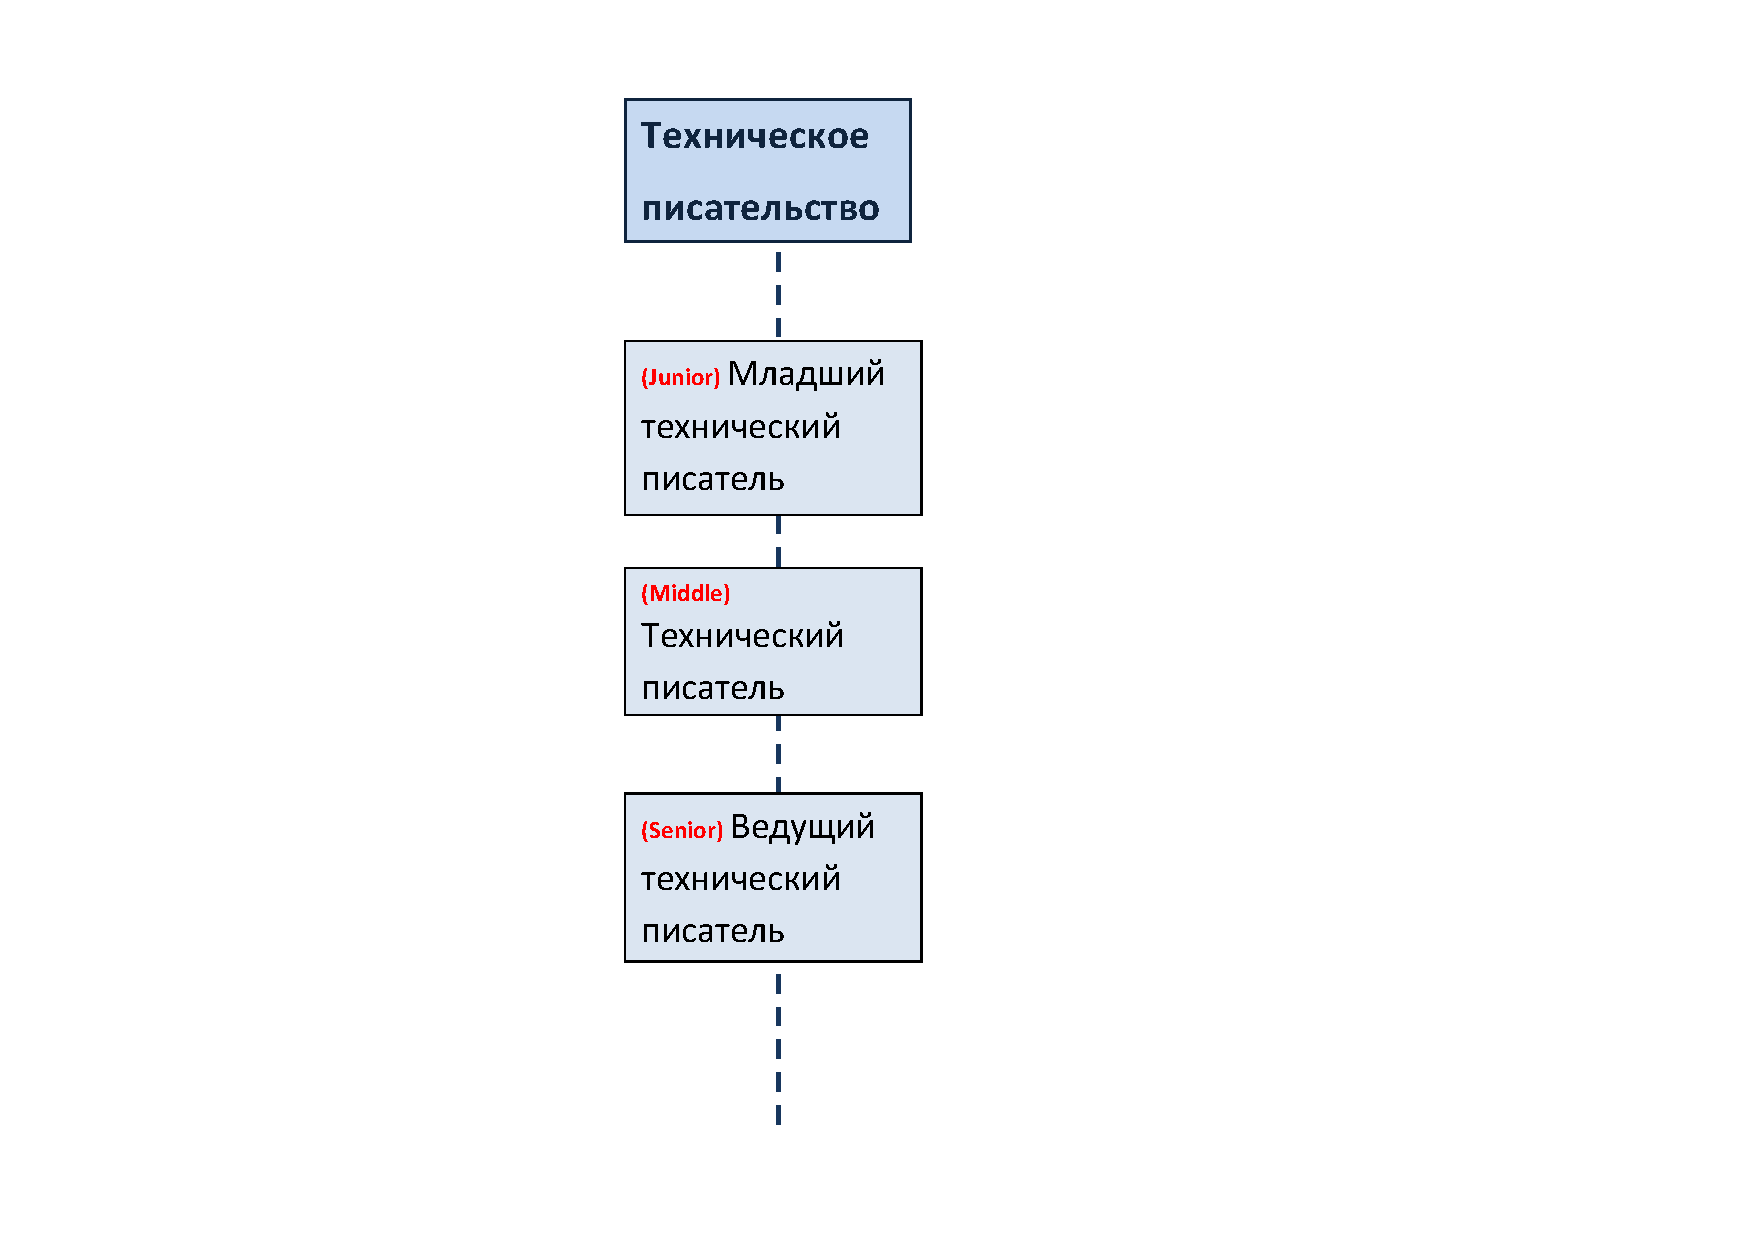
\includegraphics[width=1.11\linewidth]{11-IT-specialist's-way/schNew10.pdf}}
\end{frame}

\lecturenotes

 2ым~\cite{mc} прямым переходом  - является переход внутри сегмента, связанного с техническим писательством. Подробнее разберем далее.


\begin{frame} \frametitle{Развитие технического писателя внутри специальности: младший технический писатель }
  \begin{block}{}
  \alert{Позиция --- младший технический писатель (Junior TW) }

Должностные обязанности: 
  \end{block}
  \begin{itemize}
  \item  Разработка технической документации (руководств оператора и инженера, ПЗ, ТУ, ТЗ, технических паспортов и др.) в соответствии с требованиями  ГОСТ
  \item  Проверка и корректировка технической документации
  \item Сбор информации у всех участников процесса: заказчиков, разработчиков, инженеров
 \item Владение ИТ-терминологией и техническим английским
  \end{itemize}
\end{frame}


\lecturenotes

Позиция – Младший Технический~\cite{hh} писатель~\cite{itcf}
Обязанности~\cite{rab}:

•	Разработка, проверка и корректировка технической документации (руководств оператора и инженера, правил эксплуатации, ПЗ, ТУ, ТЗ, технических паспортов и прочих документов) в соответствии с требованиями ГОСТ 

•	Подготовка графических схем по исходным данным

•	Сбор информации у всех участников процесса: заказчиков, разработчиков, инженеров

•	Подготовка материалов технических презентаций

•	Владение ИТ-терминологией и английским;

\begin{frame} \frametitle{Развитие технического писателя внутри специальности: технический писатель }
  \begin{block}{}
  \alert{Позиция --- технический писатель (Middle TW) }

Должностные обязанности в отличие от младшего технического писателя: 
  \end{block}
  \begin{itemize}
  \item Корректировка технических заданий
  \item  Поддержание документации в актуальном состоянии
  \item Эпизодически обучение пользователей
 \item 	Согласование требований с отделом разработки
  \end{itemize}
\end{frame}


\lecturenotes

Позиция –  Технический~\cite{hh} писатель~\cite{itcf}~\cite{rab}
•	Участие в создании информационно-аналитических систем на всех этапах жизненного цикла;

•	Корректировка технических заданий, формирование UseCase;

•	Поддержание документации в актуальном состоянии

•	Эпизодически обучение пользователей;

•	Согласование требований с отделом разработки;

\begin{frame} \frametitle{Развитие технического писателя внутри специальности: ведущий технический писатель }
  \begin{block}{}
  \alert{Позиция --- ведущий технический писатель (Senior TW) }

Должностные обязанности в отличие от технического писателя: 
  \end{block}
  \begin{itemize}
  \item Управление разработкой и оценка затрат на создание комплекта технической документации
  \item Поиск путей улучшения выпускаемой технической документации
  \item Внедрение в компании средств разработки технической документации
 \item 	 Техническая поддержка разработчиков технической документации
  \end{itemize}
\end{frame}

\lecturenotes

Позиция – Ведущий Технический ~\cite{hh} писатель~\cite{itcf}
Задачи~\cite{rab}:

•	оценка затрат на создание комплекта технической документации 

•	управление разработкой комплекта технической документации

•	поиск путей улучшения выпускаемой технической документации 

•	внедрение в компании средств разработки тех. документации 

•	 техническая поддержка разработчиков технической документации


\begin{frame} \frametitle{Развитие бизнес-аналитика внутри специальности }
  \centerline{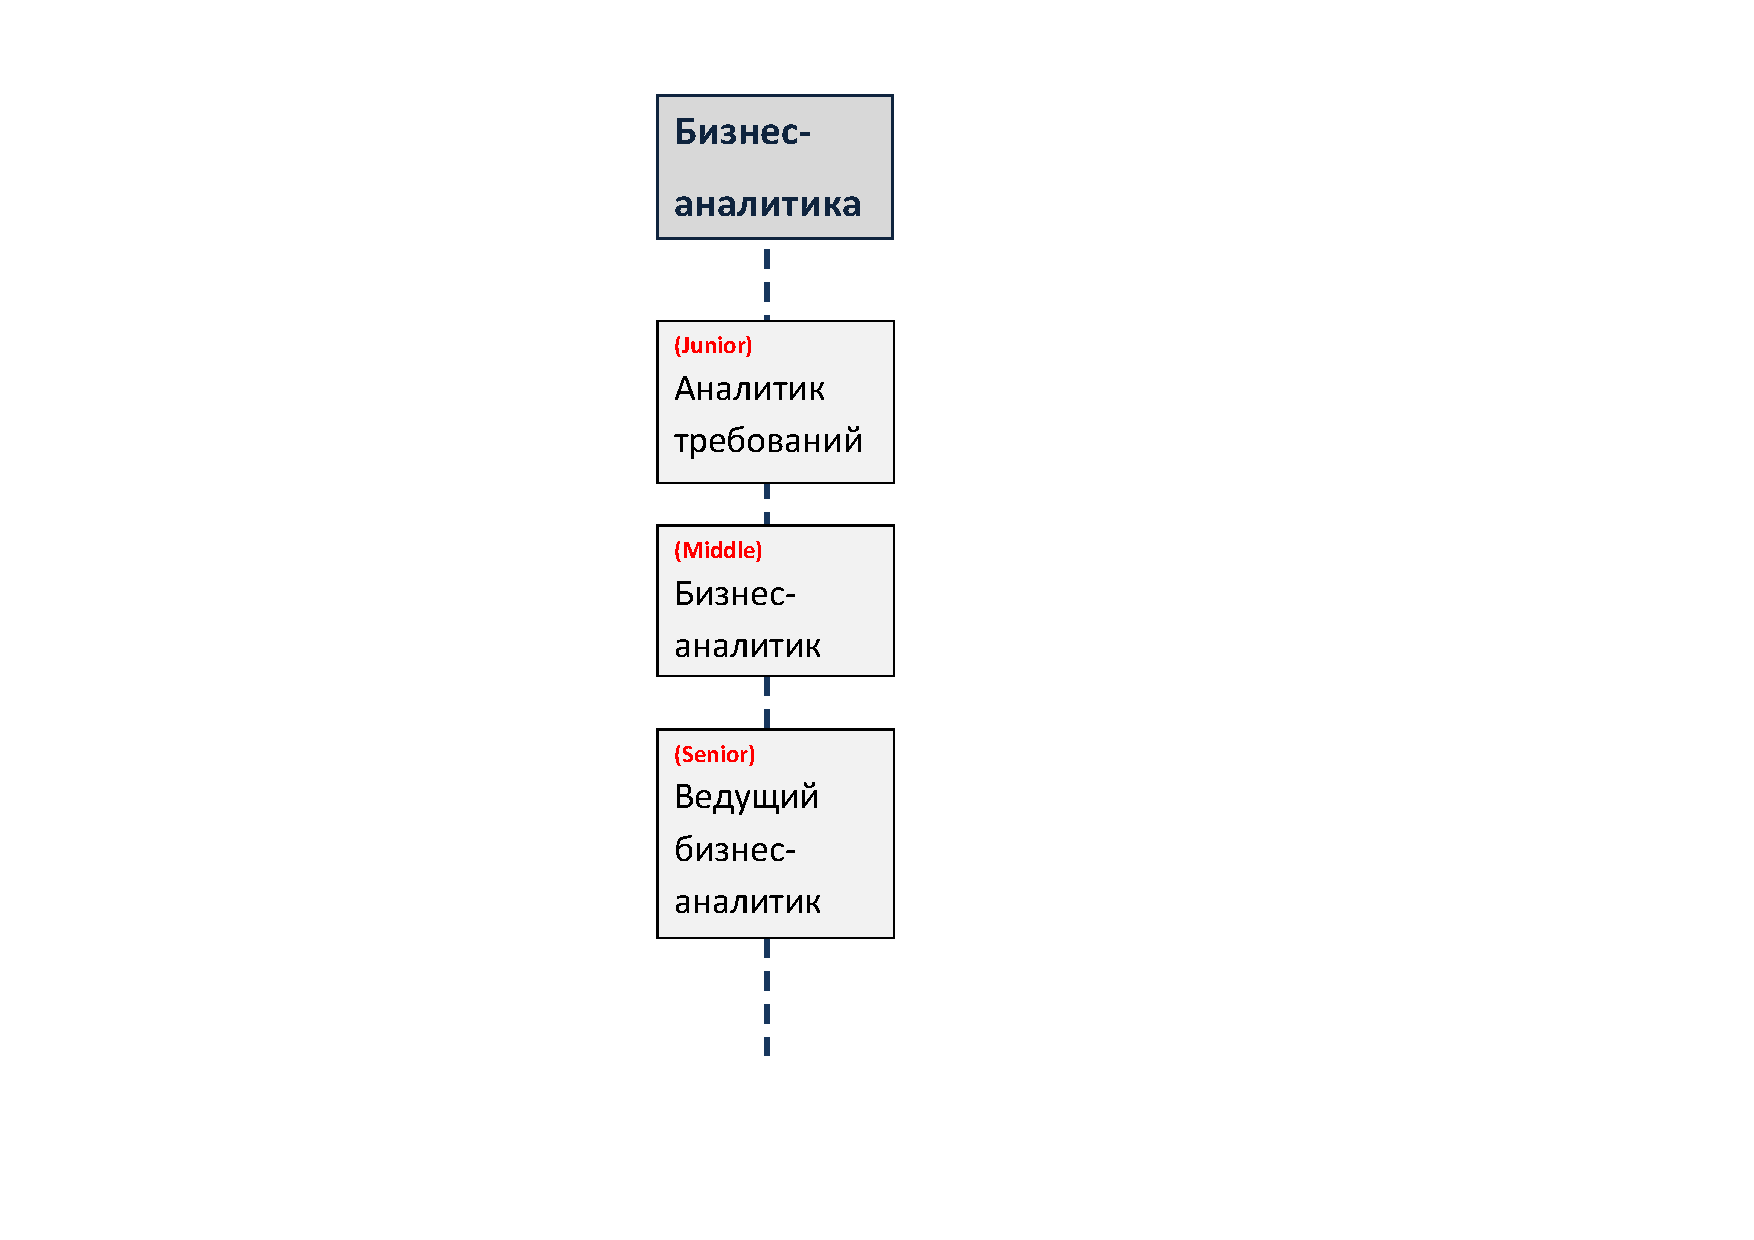
\includegraphics[width=1.27\linewidth]{11-IT-specialist's-way/schNew12.pdf}}
\end{frame}

\lecturenotes

 3им~\cite{mc} прямым переходом  - является переход внутри сегмента, связанного с работой бизнес-аналитиков. Подробнее разберем далее.

\begin{frame} \frametitle{Развитие бизнес-аналитика внутри специальности: аналитик требований }
  \begin{block}{}
  \alert{Позиция --- аналитик требований (Junior  BA) }

Должностные обязанности: 
  \end{block}
  \begin{itemize}
  \item  Настройка бизнес-процессов в системе электронного документооборота 
  \item  Сбор и формализация требований заказчика 

по автоматизации
  \item Участие в проектах по внедрению 
 \item Создание проектной документации
  \end{itemize}
\end{frame}


\lecturenotes

Позиция – Аналитик~\cite{hh} требований~\cite{itcf}
Обязанности~\cite{rab}:
•	Настройка бизнес-процессов в системе электронного документооборота 

•	Сбор и формализация требований Заказчика по автоматизации 

•	Участие в проектах по внедрению 

•	Создание проектной документации


\begin{frame} \frametitle{Развитие бизнес-аналитика внутри специальности: бизнес-аналитик}
  \begin{block}{}
  \alert{Позиция --- бизнес-аналитик (Middle  BA) }

Должностные обязанности в отличие от аналитика требований: 
  \end{block}
  \begin{itemize}
  \item  Прогнозировать спрос,анализ отклонений 

от стратегических планов
  \item  Прогноз и оценка эффективности маркетинговой деятельности
  \item Оценка результатов продуктовых изменений 

и экспериментов
 \item  Сбор, обработка и хранение данных из CRM
 \item  Информационная поддержка руководителя
  \end{itemize}
\end{frame}


\lecturenotes

Позиция~\cite{hh} –  бизнес-аналитик~\cite{itcf}

Обязанности~\cite{rab}:

	прогнозировать спрос 

Анализ отклонений от стратегических планов

Подготовка аналитических материалов, аналитических записок по деятельности компании

 Прогноз и оценка эффективности маркетинговой деятельности

Оценка результатов продуктовых изменений и экспериментов

Анализ динамики статей консолидированной финансовой отчетности

Сбор, обработка и хранение данных из CRM

 Информационная поддержка руководителя

 Подготовка презентаций, работа с таблицами, графиками и т.д.


\begin{frame} \frametitle{Развитие бизнес-аналитика внутри специальности: ведущий бизнес-аналитик}
  \begin{block}{}
  \alert{Позиция --- ведущий бизнес-аналитик (Senior  BA) }

Должностные обязанности в отличие от бизнес-аналитика: 
  \end{block}
  \begin{itemize}
  \item  Разработка и реинжиниринг бизнес-процессов компании
  \item Экспертная поддержка проектов внедрения ИТ систем в части бизнес-процессов
  \item Способствование оптимальному функционированию системы управления качеством
 \item  Обеспечение исполнения решений руководства, своевременное информирование руководства 

о текущем ходе работ и их результатах
 \item  Обучение кадров
  \end{itemize}
\end{frame}



\lecturenotes
Позиция – Ведущий~\cite{hh} бизнес-аналитик~\cite{itcf}
Обязанности~\cite{rab}:

•	Разработка и реинжиниринг бизнес-процессов в области:

первичного производственного учета,

 расчета материального баланса,

управления потерями и топливом на собственные нужды,

повышения операционной эффективности.

•         обучение кадров

•	Экспертная поддержка проектов внедрения ИТ систем в части бизнес-процессов.

•	Участие в разработке технических требований и технических заданий для реализации ИТ инструментов автоматизации обновленных бизнес-процессов.  

•	способствование оптимальному функционированию системы управления качеством;

•	Обеспечение исполнения решений руководства, своевременное информирование руководства о текущем ходе работ и их результатах.






\begin{frame} \frametitle{Косвенные переходы между специальностями: 2 часть из 4}
 \begin{block}{Технические навыки}
 Развивая \alert{технические навыки}, у специалиста появляется возможность переходов: 
\begin{itemize}
 \item Веб-разработчик ---> Разработчик
\end{itemize}
  \end{block}
  
\begin{block}{Навыки аналитики}
 Развивая \alert{навыки аналитики}, у специалиста появляется возможность переходов: 
\begin{itemize}
 \item Тестировщик ---> Бизнес-аналитик
 \item Ведущий разработчик ---> Бизнес-аналитик
 \item Проектировщик интерфейсов ---> Бизнес-аналитик
\end{itemize}
  \end{block}
\end{frame}


\begin{frame} \frametitle{Косвенные переходы между специальностями: 2 часть из 4}
 \begin{block}{Навыки дизайна}
 Развивая \alert{навыки дизайна}, у специалиста появляется возможность переходов: 
\begin{itemize}
 \item Технический писатель ---> Проектировщик интерфейсов
\end{itemize}
  \end{block}

\begin{block}{Навыки тестирования}
 Развивая \alert{навыки тестирования}, у специалиста появляется возможность переходов: 
\begin{itemize} 
 \item Технический писатель ---> Тестировщик
\end{itemize}
  \end{block}
\end{frame}


\begin{frame} \frametitle{Косвенные переходы между специальностями: мотивация }

 \begin{block}{}
Мотивы, обуславливающие данные переходы:
  \end{block}
\begin{itemize}
\item Социальный мотив (занять достойное место 

в обществе в соответствии с интересами)
\item Познавательный мотив (стремление к овладеванию специальными знаниями, проникновением 

в сущность профессиональной деятельности)
\item Эстетический мотив (желание работать по данной специальности)
\item Материальный мотив (стремление иметь более высокооплачиваемую работу) 
\item Престижный мотив (стремление к работе, обеспечивающей более быстрое продвижение 

по службе)
  \end{itemize}
\end{frame}

\lecturenotes

Выявлены несколько групп мотивов выбора профессии:



\begin{frame} \frametitle{Косвенные переходы между специальностями: технические навыки }

\begin{block}{Веб-дизайнер ---> Разработчик }

Возможно при дополнительном изучении:
  \end{block}
\begin{itemize}
  \item Принципов подготовки аналитических материалов, аналитических записок по деятельности компании
  \item Методов прогнозирования спроса и оценка эффективности маркетинговой деятельности
\item Принципов и методов анализа динамики статей консолидированной финансовой отчетности
  \end{itemize}
\end{frame}

\lecturenotes

Веб-дизайнер ---------Middle разработчик
Возможно при дополнительном изучении~\cite{rab}:
•	Software Engineering Process
•	 Изучение и понимание технологии web-серверов и серверов приложений
•	Изучение клиентских и серверных технологий , 
•	Изучение сред разработки


\begin{frame} \frametitle{Косвенные переходы между специальностями: навыки аналитики }

\begin{block}{Тестировщик ---> Бизнес-аналитик  

Ведущий разработчик ---> Бизнес-аналитик  

Проектировщик интерфейсов ---> Бизнес-аналити}

Возможно при дополнительном изучении:
  \end{block}
\begin{itemize}
  \item Методов прогнозирования спроса и оценка эффективности маркетинговой деятельности
\item Принципов и методов анализа динамики статей консолидированной финансовой отчетности
 \item Программной инженерии
  \end{itemize}
\end{frame}

\lecturenotes


Тестировщик ---------Бизнес-аналитик
Возможно при дополнительном умении~\cite{rab}:

 Подготовка аналитических материалов, аналитических записок по деятельности компании
Прогноз спроса и оценка эффективности маркетинговой деятельности
 Оценка результатов продуктовых изменений и экспериментов
Анализ динамики статей консолидированной финансовой отчетности

Ведущий разработчик ---------Бизнес-аналитик
Возможно при дополнительном умении:
•	прогнозировать спрос 
 Прогноз и оценка эффективности маркетинговой деятельности
 Анализ динамики статей консолидированной финансовой отчетности

UX Дизайнер ---------Бизнес-аналитик
Возможно при дополнительном умении:
•	прогнозировать спрос 
Подготовка аналитических материалов, аналитических записок по деятельности компании
 Прогноз и оценка эффективности маркетинговой деятельности
 Анализ динамики статей консолидированной финансовой отчетности





\begin{frame} \frametitle{Косвенные переходы между специальностями: навыки дизайна }

\begin{block}{Технический писатель ---> Проектировщик интерфейсов}

Возможно при дополнительном изучении:
  \end{block}
\begin{itemize}
  \item Принципов проектирования пользовательских сценариев
  \item Принципов и методов отрисовки интерфейса 

в графических редакторах
\item Требований к подготовке и передаче макетов разработчикам
  \end{itemize}
\end{frame}

\lecturenotes

Технический писатель ---------UX Дизайнер
Возможно при дополнительном умении~\cite{rab}:
•	проектировать пользовательских сценариев;
•	отрисовка интерфейса в графических редакторах.
•	подготовка и передача макетов для разработчиков
•	разработка стиля, составление инструкций по шрифтам, цветам и размерам;

\begin{frame} \frametitle{Косвенные переходы между специальностями: навыки тестирования}
\begin{block}{Технический писатель ---> Тестировщик}

Возможно при дополнительном изучении:
  \end{block}
\begin{itemize}
  \item Принципов проведения ручного тестирования разделов приложения
  \item Принципов создание тест-кейсов,проведение функционального и регрессивного тестирования
  \end{itemize}
\end{frame}

\lecturenotes


Технический писатель ---------Тестировщик
Возможно при дополнительном умении:
•	проведение ручного тестирования разделов приложения;
•	создание и поддержка тест-кейсов в актуальном состоянии;
•	проведение функционального и регрессивного тестирования, cоставление отчетов по итогам проведенного тестирования;
•	тестирование верстки страниц при различных сценариях поведения пользователей;
•	работа в системе баг-трекинга.




\begin{frame} \frametitle{Развитие  специалиста в иерархии компании: 3 часть из 4 }
  \centerline{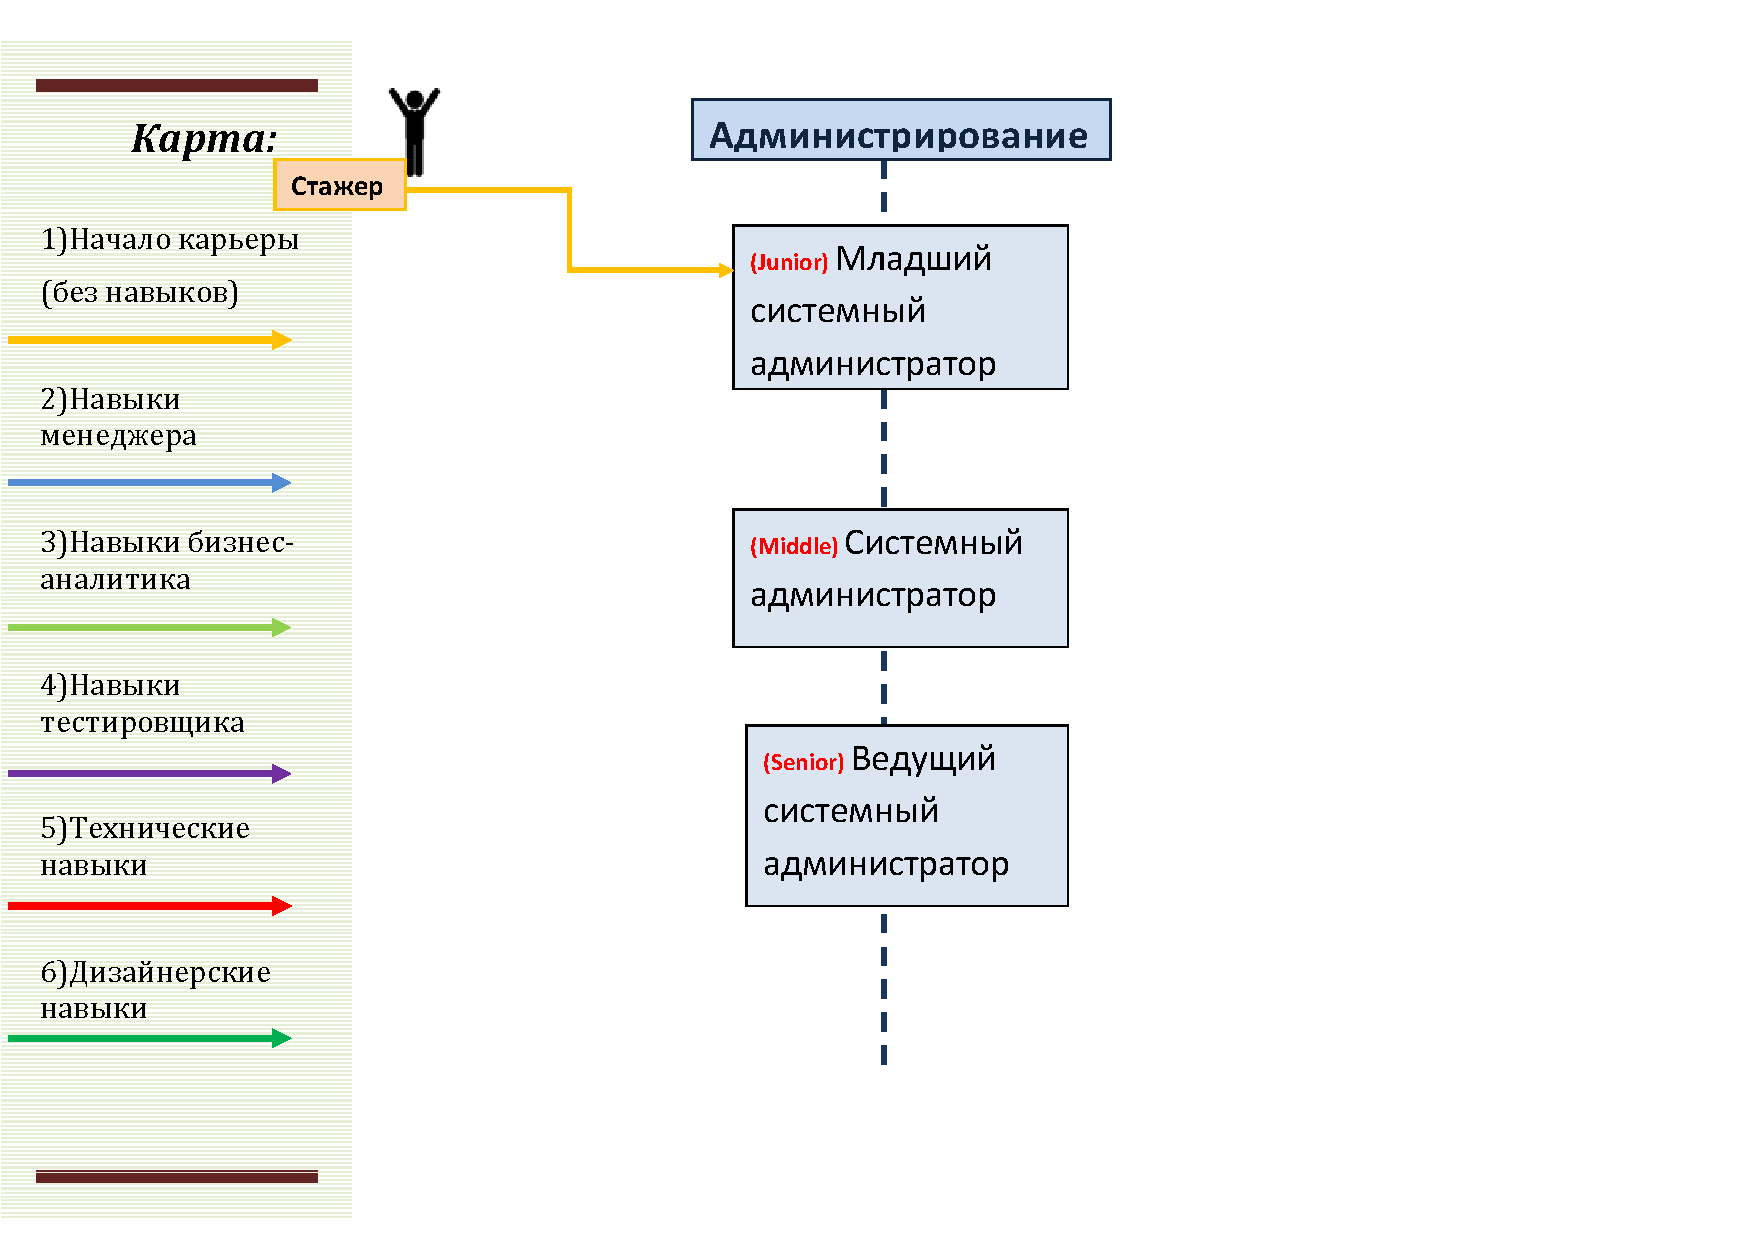
\includegraphics[width=1.13\linewidth]{11-IT-specialist's-way/schNew4.pdf}}
\end{frame}


\begin{frame} \frametitle{Развитие системного администратора внутри специальности: младший системный администратор }
 \begin{block}{}
  \alert{Позиция --- младший системный администратор 

(Junior admin)}

Должностные обязанности: 
  \end{block}
  \begin{itemize}
  \item   Администрирование рабочих станций и решение проблем пользователя
  \item  Сопровождение ИТ оборудование удаленно
  \item Быстрое и полное восстановление данных при потери части/всей информации по вине любого сотрудника
 \item Сопровождение программных продуктов
 \item Обеспечение бесперебойной работы ИТ-инфраструктуры предприятия
  \end{itemize}
\end{frame}

\lecturenotes

Позиция – Младший системный~\cite{hh} администратор~\cite{itcf}
Задачи~\cite{rab}:

•	Администрирование рабочих станций и решение проблем пользователя

•	Сборка, установка и настройка ПК

•	сопровождение ИТ оборудование удаленно

•	Сборка образов ОС Linux, Windows

•	Выполнение регламентных работ

•	Обслуживание, установка и переустановка офисной оргтехники, обеспечение ее высокопродуктивной деятельности

•	Поиск хорошего программного обеспечения, его установка, корректировка его деятельности; обеспечение постоянной бесперебойной работы сети компании

•	Быстрое и полное восстановление данных при потери части или всей информации по вине любого из сотрудников

•	Настройка, поддержка и модернизация локальной сети

•	Техническая поддержка пользователей

•	Сопровождение программных продуктов (таких как: 1С)

•	Обеспечение бесперебойной работы ИТ-инфраструктуры предприятия

\begin{frame} \frametitle{Развитие системного администратора внутри специальности: старший системный администратор }
 \begin{block}{}
  \alert{Позиция --- системный администратор (Middle admin)}

Должностные обязанности в отличие от младшего системного администратора: 
  \end{block}
  \begin{itemize}
  \item   Развёртывание, настройка и поддержание серверов, систем хранения данных, операционных систем

 и так далее
  \item Навыки работы с виртуальными средами, контейнерными технологиями
  \item Обучение кадров
 \item Выявление потенциальных проблем, анализ текущей работы серверов и системного ПО
  \end{itemize}
\end{frame}

\lecturenotes

Позиция – Системный~\cite{hh} администратор~\cite{itcf}
Обязанности~\cite{rab}:

- развёртывание, настройка и поддержание серверов, систем хранения данных, операционных систем и т.п.

- навыки работы с виртуальными средами, контейнерными технологиями;

- Обучение кадров;

-выявление потенциальных проблем, анализ текущей работы серверов и системного ПО.

\begin{frame} \frametitle{Развитие системного администратора внутри специальности: ведущий системный администратор }
 \begin{block}{}
  \alert{Позиция --- ведущий системный администратор (Senior admin)}

Должностные обязанности в отличие от  системного администратора: 
  \end{block}
  \begin{itemize}
  \item   Руководство и планирование работы отдела
  \item  Разработка предложений по развитию инфраструктуры сети
  \item Подготовка предложений по модернизации 

и приобретению сетевого оборудования, в том числе участие в составлении технических заданий на закупку оборудования
  \end{itemize}
\end{frame}

\lecturenotes

Позиция – Ведущий Системный~\cite{hh} админ~\cite{itcf}

Обязанности~\cite{rab}:

•	Руководство и планирование работы отдела.

•	Разработка предложений по развитию инфраструктуры сети.

•	Подготовка предложений по модернизации ~и приобретению сетевого оборудования, в том числе участие в составлении технических заданий на закупку оборудования



\begin{frame} \frametitle{Развитие  специалиста в иерархии компании: 4 часть из 4 }
  \centerline{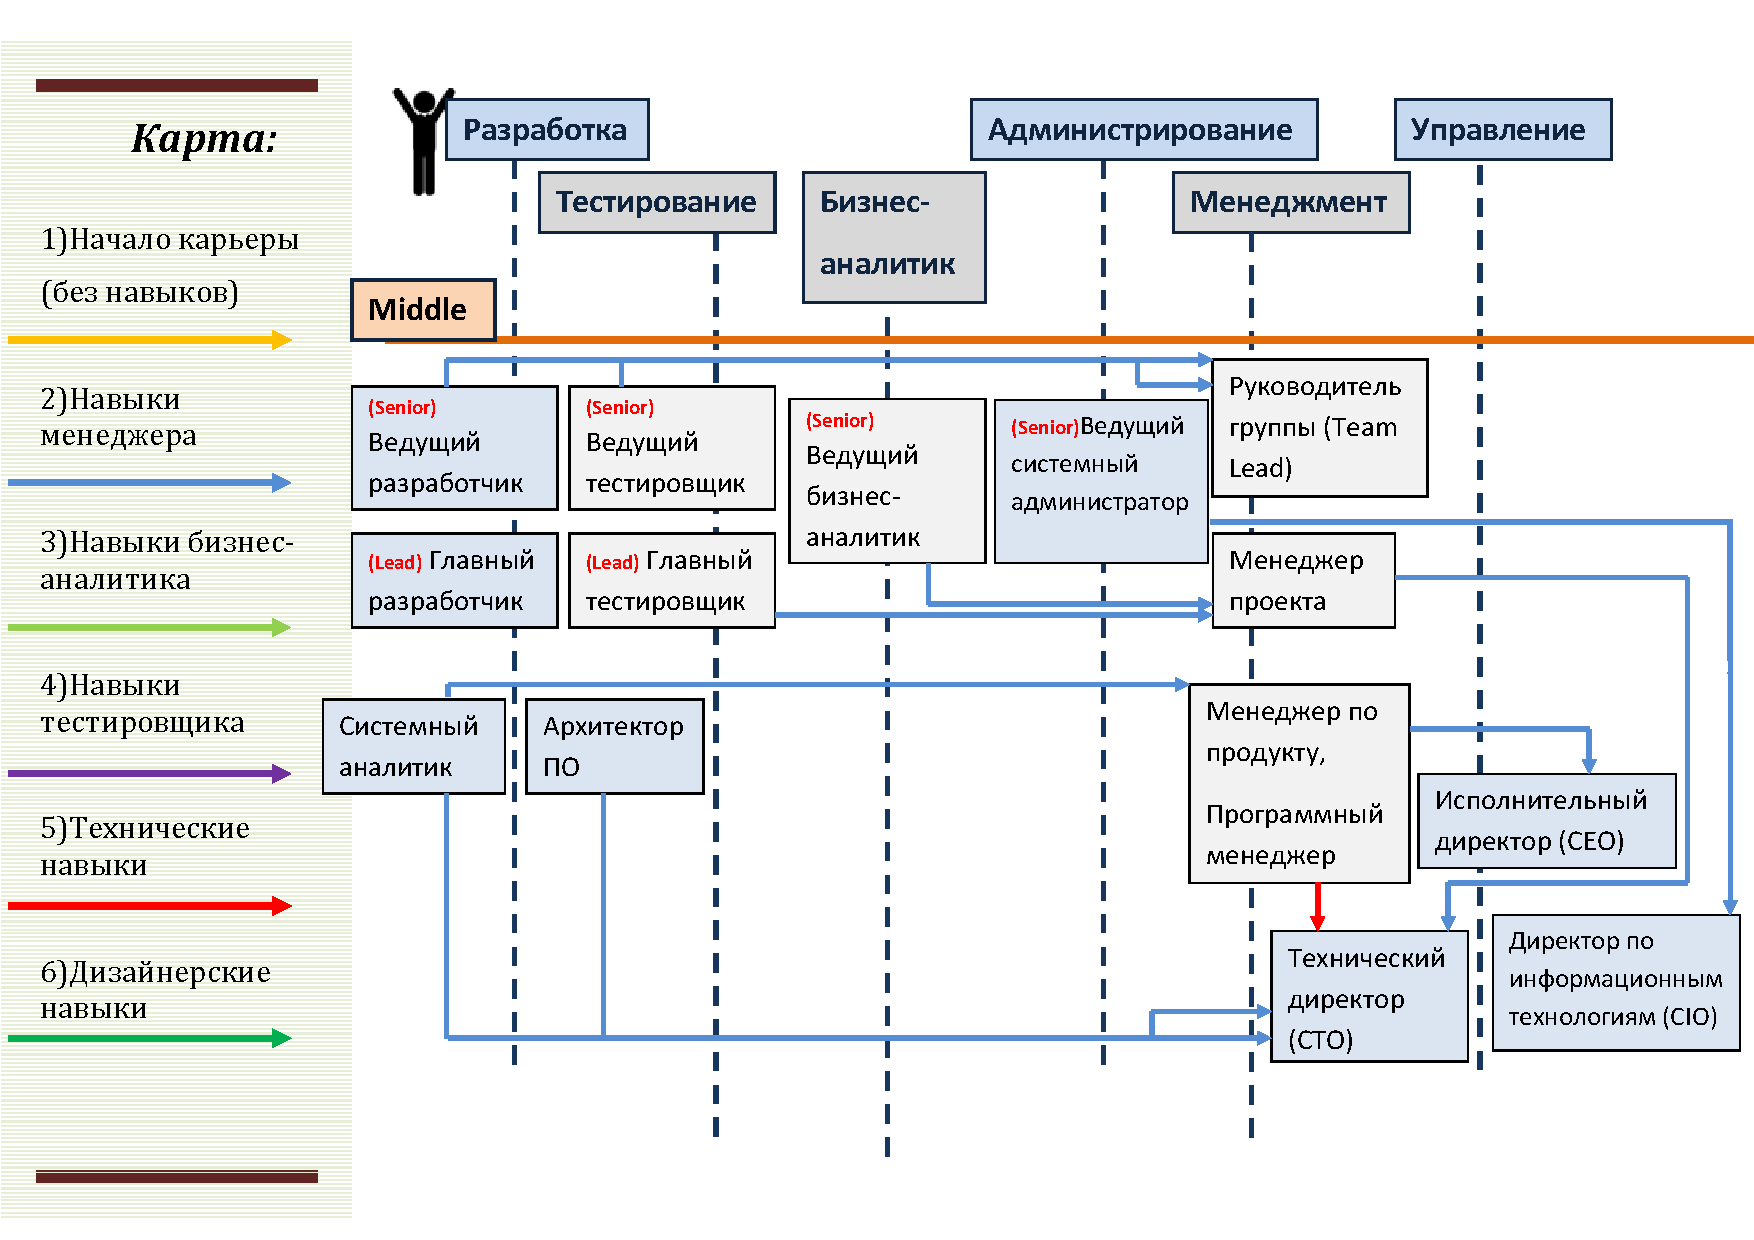
\includegraphics[height=0.93\textheight]{11-IT-specialist's-way/schNew1.pdf}}
\end{frame}


\begin{frame} \frametitle{Развитие управляющего персонала внутри специальности}
  \centerline{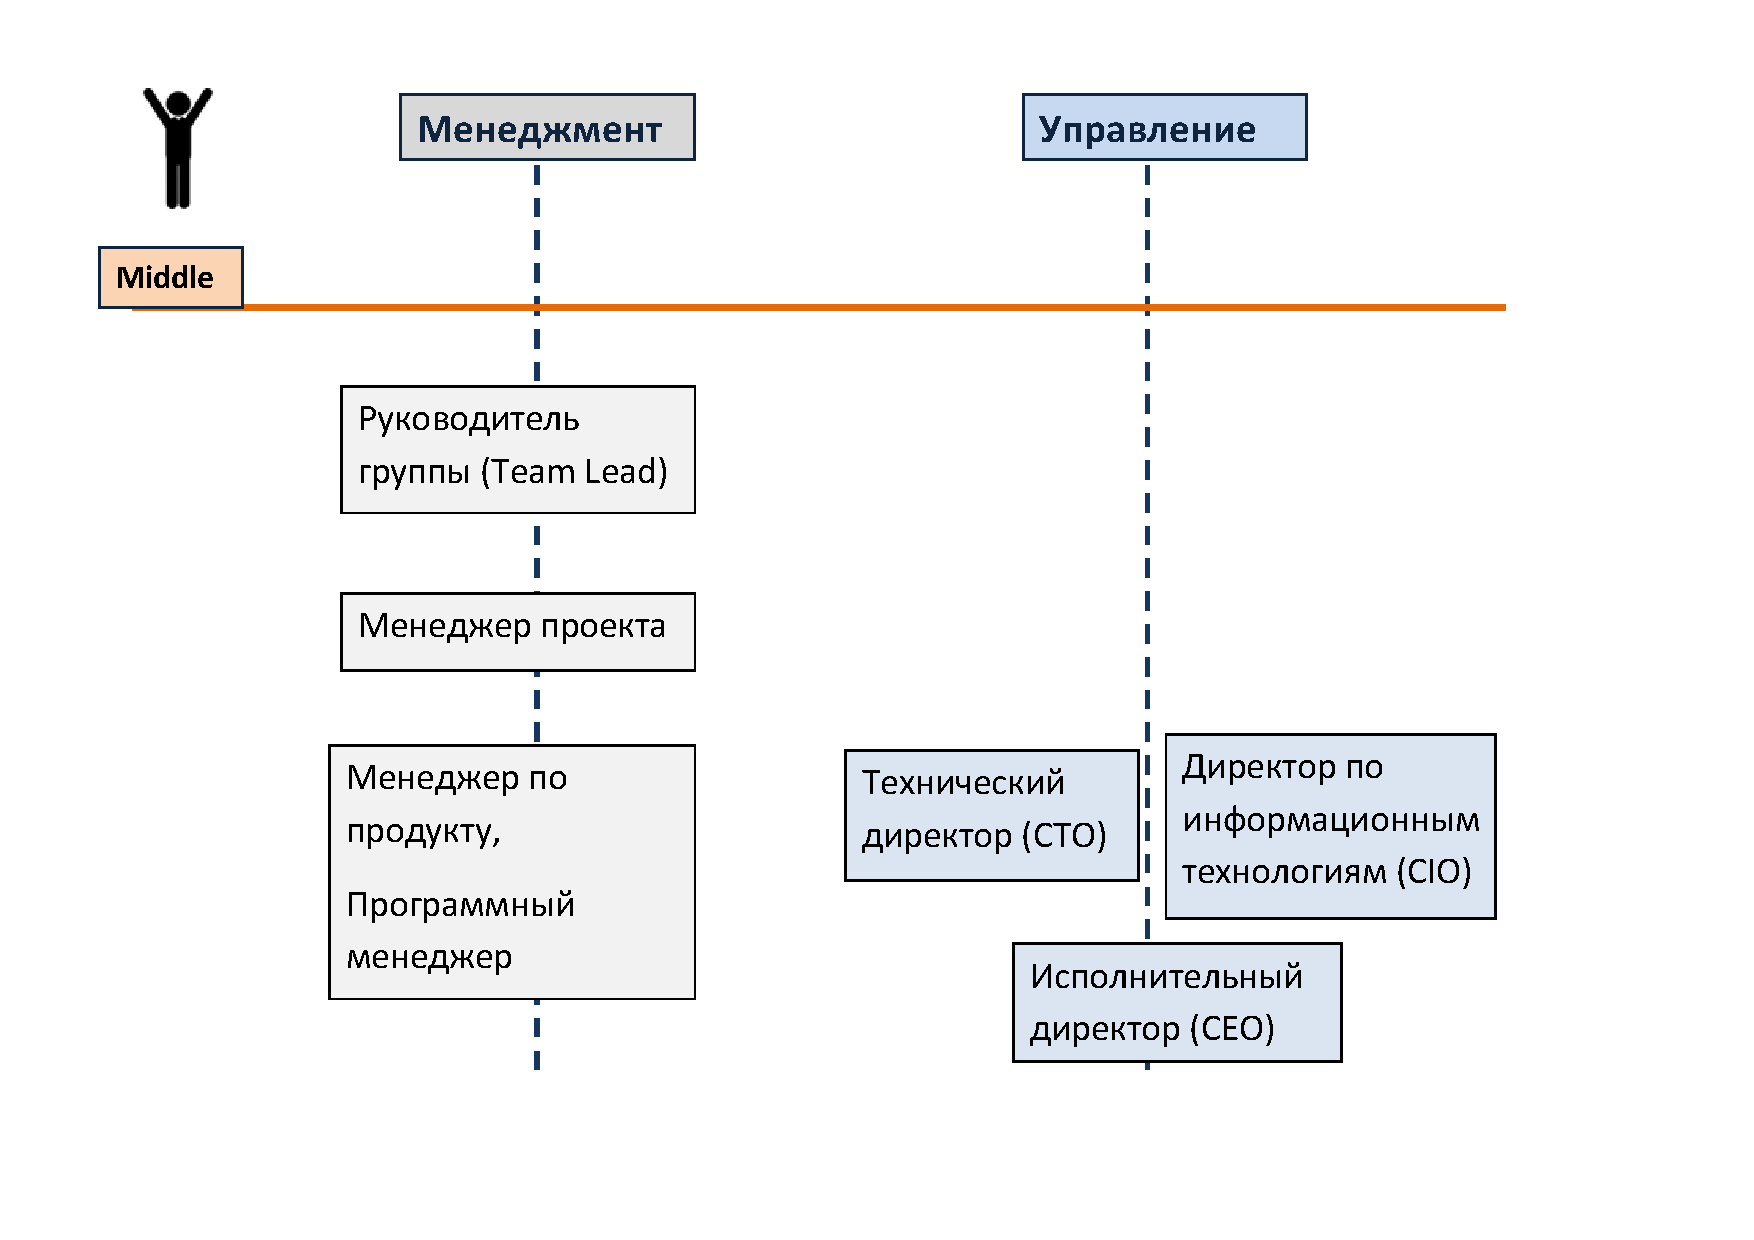
\includegraphics[width=1.14\linewidth]{11-IT-specialist's-way//schNew51.pdf}}
\end{frame}
\lecturenotes

 1 прямый~\cite{mc} переход  -  менеджмент. Далее рассмотрим подробнее



\begin{frame} \frametitle{Развитие управляющего персонала внутри специальности: руководитель группы}
 \begin{block}{}
  \alert{Позиция --- руководитель группы (Team Lead)}

Должностные обязанности в отличие от главных (разработчиков, тестировщиков, бизнес-аналитиков, системных администраторов и т.д.): 
  \end{block}
  \begin{itemize}
  \item Управление версиями проекта
  \item Подбор команды для реализации проекта,обучение персонала
 \item  Переговоры с клиентами, подготовка коммерческих предложений, проведение презентаций
  \item Составление отчетности для руководства
  \end{itemize}
\end{frame}

\lecturenotes

Позиция – Руководитель~\cite{hh} группы~\cite{itcf}

Обязанности~\cite{rab}:

- Управление отделом backend-разработки;

- Организация процесса разработки;

- Прототипирование;

- Разработка архитектуры системы;

- Трансформация use case/ spring tasks;

- Создание дизайн-моделей на базе т.з. и use case / user story;

- Написание API;

- Моделирование структуры хранения в базах данных

- Разработка функционала End-to-End;

- Code review;

- Документирование;

- Обучение членов команды.

- Организация взаимодействия с отделами аналитики, тестирования, администрирования;

- Unit - тесты;

- Ведение backlog;

- Управление версиями проекта;

- Подбор команды для реализации проекта;

- Переговоры с клиентами, подготовка коммерческих предложений, проведение презентаций;

- Составление отчетности для руководства;

\begin{frame} \frametitle{Развитие управляющего персонала внутри специальности: менеджер проекта}
 \begin{block}{}
  \alert{Позиция --- менеджер проекта (Project manager)}

Должностные обязанности в отличие от руководителя группы: 
  \end{block}
  \begin{itemize}
  \item Разработка плана управления проектом,детального дизайна проекта

  \item Определение содержания проекта и разработка устава

 \item Планирование и управление рисками, контроль бюджета и сроков

  \item Мониторинг и управление работами проекта
  \end{itemize}
\end{frame}

\lecturenotes

Позиция –менеджер~\cite{hh} проектов~\cite{itcf}
Обязанности~\cite{rab}:

 • Разработка плана управления проектом;

• Разработка детального дизайна;

• Определение содержания проекта;

• Разработка устава проекта;

• Планирование и управление рисками;

• Управление изменениями проекта;

• Мониторинг и управление работами проекта;

• Контроль и управление качеством предоставляемых на проекте услуг;

• Контроль бюджета и сроков проекта;



\begin{frame} \frametitle{Развитие управляющего персонала внутри специальности:  программный менеджер, менеджер по продукту}
 \begin{block}{}
  \alert{Позиция --- менеджер по продукту (Product Manager)}

Должностные обязанности в отличие от менеджера проекта: 
  \end{block}
  \begin{itemize}
  \item Построение стратегии продвижения приложения 

на англоязычные рынки
  \item Управлять полным продуктовым циклом
 \item Определять цели и KPI, а позже достижение их вместе с командой
  \end{itemize}
\end{frame}

\lecturenotes

Позиция~\cite{hh} – менеджер по продукту~\cite{itcf}~\cite{rab}
•	Управление процессом развития стартап проекта 

•	Осуществление маркетингового анализа и исследований (изучение рынка, конкурентов и пр.).

•	Построение стратегии продвижения приложения на англоязычные рынки

•	Создание прототипов пользовательского интерфейса 

•	Управлять полным продуктовым циклом, совмещая роли product и project менеджера: искать и анализировать идеи, писать понятные технические задания, ставить задачи на разработку, расставлять приоритеты, планировать ресурсы, контролировать сроки и качество исполнения, анализировать полученные результаты;

•	Определять цели и KPI, а потом достигать их вместе с командой;



\begin{frame} \frametitle{Развитие управляющего персонала внутри специальности:  программный менеджер,  менеджер по продукту}
 \begin{block}{}
  \alert{Позиция --- программный менеджер (Program Manager)}

Должностные обязанности в отличие от менеджера проекта: 
  \end{block}
  \begin{itemize}
  \item Осуществляет выбор оптимального сочетания потребностей пользователей и возможностей информационной системы
 \item Управление заявками пользователей на обслуживание
 \item Осуществляет прогнозирование изменений 

в автоматизации предприятия и разрабатывает меры упреждающего управления
  \end{itemize}
\end{frame}

\lecturenotes

Позиция – программный~\cite{hh} менеджер~\cite{itcf}~\cite{rab}

1.	Осуществляет выбор оптимального сочетания потребностей пользователей и возможностей информационной системы.

2.	Разрабатывает методологическую основу информационной системы.

3.	Организует подготовку проектной документации, сметы расходов на информационную систему и ее функционирование.

4.	Руководит работами по настройке и поддержке информационной системы.

5.	Осуществляет:
1.	7.1. Контроль и установку программного обеспечения (software control and distribution).
2.	7.3. Управление заявками пользователей на обслуживание (incident management).
3.	7.4. Управление изменениями (change management):
o	управление запросами на изменения (RfC);
o	подтверждение и планирование изменений;
o	управление приоритетами запросов.
4.	7.5. Управление составом ИС (сonfiguration management):
o	контроль инфраструктуры посредством поддержки адекватных данных обо всех необходимых ресурсах;
o	предоставление текущего статуса и истории каждого элемента инфраструктуры;
o	взаимосвязь элементов инфраструктур.
5.	7.6. Управление надежностью (availability management).
6.	7.7. Устранение нарушений работы сервисов (problem management).

6.	Осуществляет прогнозирование изменений в автоматизации предприятия и разрабатывает меры упреждающего управления.


\begin{frame} \frametitle{Управляющий персонал внутри специальности: технический директор}
 \begin{block}{}
  \alert{Позиция --- технический директор (CTO)}

Должностные обязанности: 
  \end{block}
  \begin{itemize}
  \item Контроль выполнения плана производства; определение контрольных точек; ритмичный выпуск продукции
 \item Разработка и согласование расчетов производственных мощностей, технологических планировок и  процессов, подборе, комплектации 

и модернизации оборудования производства
 \item Контроль организации и проведение работ 

в  подразделениях в соответствии с утвержденными технологическими регламентами, схемами, обеспечивать правильную эксплуатацию оборудования 
  \end{itemize}
\end{frame}

\lecturenotes

Позиция – CTO, технический~\cite{hh} директор~\cite{itcf}

•	Обязанности~\cite{rab}:

Управление службами

o	Технологический отдел
o	ПДО
o	Служба механика
o	Производство
o	ОТК

•	Контроль выполнения плана производства; определение контрольных точек для осуществления контроля процесса производства; ритмичный выпуск продукции

•	Разработка и согласование расчетов производственных мощностей, технологических планировок и технологических процессов, подборе, комплектации и модернизации оборудования производства, в освоении новых технологий;

•	Разработка и внедрение производственных процессов с целью повышения производительности и качества выпускаемой продукции.

•	Составление инвестиционных планов по техническому обеспечению.

•	Внедрение современных стратегий сокращения издержек производства; Участие в разработке проектов, направленных на улучшение организации производства.

•	Организовывать рациональное использование производственных ресурсов: полное использование имеющихся мощностей, рациональная загрузка и уменьшение простоев оборудования;

•	Организовывать текущее производственное планирование, учет, составление и своевременное представление отчетности о производственной деятельности подчиненных подразделений, организовывать работу по правильному применению форм и систем заработной платы и материального стимулирования.

•	Организовывать контроль за внесением изменений, анализировать изменения на качество продукции;

•	Организовывать и обеспечивать подготовку производства к прохождению внутренних и внешних проверок.

•	Контролировать организацию и проведение работ в подчиненных подразделениях в соответствии с утвержденными технологическими регламентами, картами, схемами, обеспечивать технически правильную эксплуатацию оборудования и других основных средств

•	Координировать работу цехов и функциональных служб подчиненных подразделений, определять полномочия, должностные обязанности и ответственность подчиненного персонала.

•	Анализировать деятельность подчиненных подразделений и результаты анализа доводить до сведения генерального директора


\begin{frame} \frametitle{Управляющий персонал внутри специальности: исполнительный директор}
 \begin{block}{}
  \alert{Позиция --- исполнительный директор (CEO)}

Должностные обязанности: 
  \end{block}
  \begin{itemize}
  \item Организация работ и взаимодействия всех подразделений компании
 \item Оперативное выполнение анализа деятельности
 \item Проверка правильности делопроизводства: смотрит 

за соблюдением норм экономического и юридического делопроизводства
  \item Выполняет поручения непосредственного руководителя --- генерального директора
  \end{itemize}
\end{frame}

\lecturenotes

Позиция –CEO, исполнительный~\cite{hh} директор~\cite{itcf}
Обязанности~\cite{rab}:

•	Организация работ и взаимодействия всех подразделений компании. 

•	Участие в развитии и стратегическом планировании деятельности предприятия. 

•	Оперативное выполнение анализа деятельности. 

•	Разработка системы мотивирующих стимулов для работников. 

•	Отвечает за соблюдение его подчиненными правил трудовой дисциплины. 

•	Проверка правильности делопроизводства: смотрит за соблюдением норм экономического и юридического делопроизводства.

•	 Выявляет недостатки в деятельности компании и предпринимает все возможные средства для устранения недостатков в работе. 

•	Выполняет поручения непосредственного руководителя - генерального директора. 


\begin{frame} \frametitle{Управляющий персонал внутри специальности: директор по информационным технологиям }
 \begin{block}{}
  \alert{Позиция --- директор по информационным технологиям (CIO)}

Должностные обязанности: 
  \end{block}
  \begin{itemize}
  \item Разработка модели монетизации проекта
 \item Постановка и распределение задач между подразделениями
\item Контроль сроков/стоимости/качества выполнения работ
 \item Разработка стратегии продвижения и рекламы продукта
  \itemМодернизация IT-инфраструктуры компании
  \end{itemize}
\end{frame}

\lecturenotes

	Позиция –CIO, Директор по информационным~\cite{hh} технологиям~\cite{itcf}

Обязанности~\cite{rab}:

- Разработка модели монетизации проекта;

- Оценка сроков и стоимости реализации системы;

- Разработка архитектуры развёртывания приложения;

- Разработка документации по проекту;

- Подбор исполнителей;

- Постановка и распределение задач;

- Контроль сроков/стоимости/качества выполнения работ;

- Организация непрерывного тестирования продукта;

- Разработка стратегии продвижения и рекламы продукта;

- Организация технической поддержки продукта.

- Подбор и обучение сотрудников;

- Модернизация IT-инфраструктуры компании.

\begin{frame} \frametitle{Косвенные переходы между специальностями: 4 часть из 4}
 \begin{block}{Технические навыки}
 Развивая \alert{технические навыки}, у специалиста появляется возможность переходов: 
\begin{itemize}
  \item Программный менеджер ---> Технический директор
  \item Менеджер по продукту ---> Технический директор
  \end{itemize}
  \end{block}
\begin{block}{Навыки необходимые для менеджера}
 Развивая \alert{навыки необходимые для менеджера}, 

у специалиста появляется возможность переходов: 
\begin{itemize}
  \item Ведущий разработчик ---> Руководитель группы
  \item Ведущий тестировщик ---> Руководитель группы
\item Главный тестировщик---> Менеджер проекта
  \end{itemize}
  \end{block}
\end{frame}

\begin{frame} \frametitle{Косвенные переходы между специальностями: 4 часть из 4}
 \begin{block}{Навыки необходимые для менеджера}
Развивая \alert{навыки необходимые для менеджера}, 

у специалиста появляется возможность переходов: 
\begin{itemize}
 \item Ведущий бизнес-аналитик ---> Менеджер проекта
  \item Архитектор ПО  ---> Технический директор
\item  Системный аналитик ---> Технический директор
 \item Системный аналитик ---> Программный менеджер
 \item Системный аналитик ---> Менеджер по продукту
\item  Программный менеджер ---> Исполнительный директор
\item Менеджер по продукту  ---> Исполнительный директор
  \end{itemize}
  \end{block}

\end{frame}


\begin{frame} \frametitle{Косвенные переходы между специальностями: мотивация }

 \begin{block}{}
Мотивы, обуславливающие данные переходы:
  \end{block}
\begin{itemize}
\item Социальный мотив (занять достойное место 

в обществе в соответствии с интересами 

и возможностями)
\item Эстетический мотив (желание работать по данной специальности)
\item Материальный мотив (стремление иметь более высокооплачиваемую работу, льготы) 
\item Престижный мотив (стремления, позволяющие достичь видного положения в обществе)
  \end{itemize}
\end{frame}

\lecturenotes

Выявлены несколько групп мотивов выбора профессии:



\begin{frame} \frametitle{Косвенные переходы между специальностями: технические навыки}

\begin{block}{Программный менеджер ---> Технический директор  

Менеджер по продукту ---> Технический директор }

Возможно, развивая технические навыки, 

при дополнительном изучении:
  \end{block}
\begin{itemize}
  \item Принципов создание, контроля и ведения плана производства
  \item Принципов разработки и согласования расчетов производственных мощностей, технологических планировок и технологических процессов
\item Принципов составления инвестиционных планов 

по техническому обеспечению
  \end{itemize}
\end{frame}

\lecturenotes

Программный менеджер, Менеджер по продукту ---------CTO (технический директор)
Возможно при дополнительном изучении~\cite{rab}:
 
•	Управление службами
	Технологический отдел
	ПДО
Служба механика
	Производство
	ОТК
•	Контроль выполнения плана производства; определение контрольных точек для осуществления контроля процесса производства; ритмичный выпуск продукции
•	Разработка и согласование расчетов производственных мощностей, технологических планировок и технологических процессов, подборе, комплектации и модернизации оборудования производства, в освоении новых технологий;
•	Составление инвестиционных планов по техническому обеспечению.
•	Организовывать и обеспечивать подготовку производства к прохождению внутренних и внешних проверок.
•	Анализировать деятельность подчиненных подразделений и результаты анализа доводить до сведения генерального директора


\begin{frame} \frametitle{Косвенные переходы между специальностями: навыки необходимые менеджеру}

\begin{block}{Ведущий разработчик ---> Руководитель группы  

Ведущий тестировщик ---> Руководитель группы }

Возможно, развивая навыки необходимые менеджеру, 

при дополнительном изучении:
  \end{block}
\begin{itemize}
  \item Принципов управления отделом backend-разработки
\item Принципов подбора команды для реализации проекта
\item Требований к подготовке коммерческих предложений, проведение презентаций
  \item Требований к обеспечению взаимодействия с отделами аналитики, тестирования, администрирования
  \end{itemize}
\end{frame}

\lecturenotes

Сравниваем между собой задачи Ведущий разработчик ---> Руководитель группы  и
Ведущий тестировщик ---> Руководитель группы

\begin{frame} \frametitle{Косвенные переходы между специальностями: навыки необходимые менеджеру}

\begin{block}{Главный тестировщик---> Менеджер проекта 

 Ведущий бизнес-аналитик ---> Менеджер проекта}

Возможно, развивая навыки необходимые менеджеру, 

при дополнительном изучении:
  \end{block}
  \begin{itemize}
  \item Принципов разработки плана управления проектом, детального дизайна проекта
  \item Принципов разработка устава
 \item Методов планирования и управления рисками, контроля бюджета и сроков
  \end{itemize}
\end{frame}

\lecturenotes

Сравниваем между собой задачи Главный тестировщик---> Менеджер проекта и
 Ведущий бизнес-аналитик ---> Менеджер проекта


\begin{frame} \frametitle{Косвенные переходы между специальностями: навыки необходимые менеджеру}

\begin{block}{Архитектор ПО  ---> Технический директор  

Системный аналитик ---> Технический директор }

Возможно, развивая навыки необходимые менеджеру, 

при дополнительном изучении:
  \end{block}
  \begin{itemize}
  \item Требований к контролю выполнения плана производства, определению контрольных точек
 \item Принципов согласования расчетов производственных мощностей, технологических планировок и  процессов, комплектации ~и модернизации оборудования 
 \item Требований к контролю организации и проведению работ в  подразделениях в соответствии 

с технологическими регламентами, схемами, обеспечивать правильную эксплуатацию оборудования 
  \end{itemize}
\end{frame}



\lecturenotes
Сравниваем между собой задачи Архитектор ПО  ---> Технический директор  и
Системный аналитик ---> Технический директор


\begin{frame} \frametitle{Косвенные переходы между специальностями: навыки необходимые менеджеру}

\begin{block}{Системный аналитик ---> Программный менеджер}

Возможно, развивая навыки необходимые менеджеру, 

при дополнительном изучении:
  \end{block}
\begin{itemize}
\item Принципов и сетодов анализа оптимального сочетания потребностей пользователей 

и возможностей информационной системы
\item Методов прогнозирования изменений 

в автоматизации предприятия
 \item Методов разработки мер упреждающего управления
\end{itemize}

\end{frame}

\lecturenotes

Сравниваем между собой задачи Системный аналитик ---> Менеджер по продукту 

\begin{frame} \frametitle{Косвенные переходы между специальностями: навыки необходимые менеджеру}

\begin{block}{Системный аналитик ---> Менеджер по продукту  }

Возможно, развивая навыки необходимые менеджеру, ~при дополнительном изучении:
  \end{block}
\begin{itemize}
\item Принципов и методов построения стратегии продвижения приложения ~на англоязычные рынки
\item Принципов управления полным продуктовым циклом
\item Методов определения дальнейших целей и KPI
\end{itemize}

\end{frame}

\lecturenotes

Системный аналитик ---> Менеджер по продукту


\begin{frame} \frametitle{Косвенные переходы между специальностями: навыки необходимые менеджеру}

\begin{block}{Программный менеджер ---> Исполнительный директор 

Менеджер по продукту  ---> Исполнительный директор }

Возможно, развивая навыки необходимые менеджеру, 

при дополнительном изучении:
  \end{block}
 \begin{itemize}
  \item Принципов организации работ и взаимодействия всех подразделений компании
 \item Методов оперативного выполнения анализа деятельности
 \item Методов проверки правильности делопроизводства
  \end{itemize}
\end{frame}



\lecturenotes

Сравниваем между собой задачи Программный менеджер ---> Исполнительный директор и
Менеджер по продукту  ---> Исполнительный директор



%\section{}

\section{Взаимосвязь интересов компании и интересов сотрудника }

\subsection{3.1 Интересы компании и интересы сотрудников }

\begin{frame} \frametitle{Интересы компании и интересы сотрудников}


 \begin{table}[H]
\caption{\label{tab:canonsummary} Вопросы, на которые компании и сотруднику важно получить ответ }
\begin{center}
\begin{tabular}{|p{0.5\linewidth}|p{0.5\linewidth}|}
\hline
\textbf{Сотрудник} & \textbf{Компания} \\
\hline
В каком направлении я хочу развиваться? Каковы мои цели? &  Как увязать цели сотрудника с целями компании? \\
\hline
Где ещё я хотел бы реализовать себя?  & Как использовать потенциал сотрудников максимально? \\
\hline
Что меня вдохновляет работать с полной отдачей? & Как повысить мотивацию персонала? \\
\hline
Чему я хочу научиться? & Как улучшить качество обучения сотрудников? \\
\hline
\end{tabular}
\end{center}
\end{table} 

\end{frame}


\lecturenotes

Вопросы~\cite{IPl}, на которые компании и сотруднику важно получить ответы(рисунок).

Для того чтобы ответить на вопросы представленные на картинке, важно понять, в чем состоит главный принцип удержания ценных сотрудников.


\begin{frame} \frametitle{Взаимосвязь интересов компании и интересов сотрудника}
  \begin{block}{Главный принцип удержания ценных сотрудников}
Удержать сотрудника можно, только объединив интересы Компании с интересами этого сотрудника
  \end{block}
  \centerline{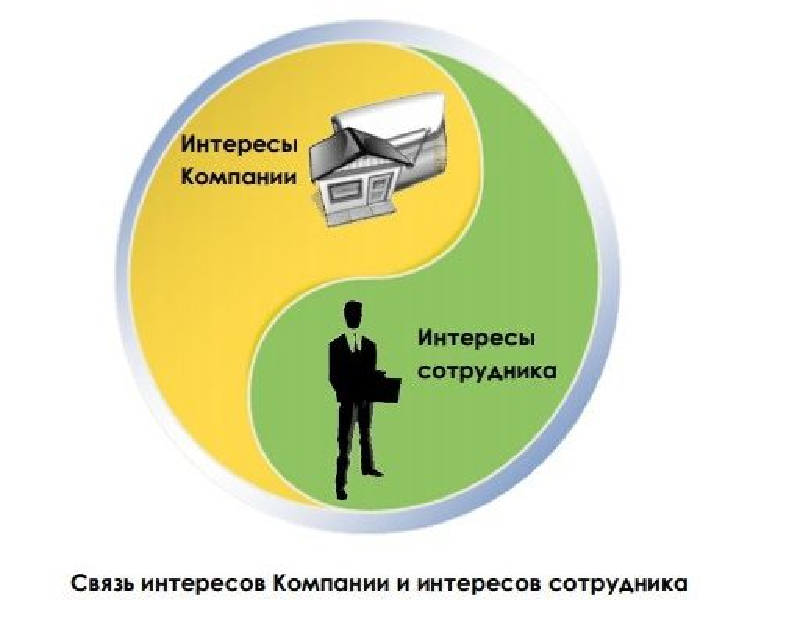
\includegraphics[height=0.58\textheight]{11-IT-specialist's-way/inter.pdf}}
\end{frame}

\lecturenotes

Главный~\cite{IPl} принцип удержания ценных сотрудников гласит, что удержать сотрудника можно, только объединив интересы Компании с интересами этого сотрудника.

Только при выполнение главного принципа удержания ценных сотрудников схемы мотивации компании будут работать, программы обучения действительно приносить приносить пользу и сотруднику и компании,а сам сотрудник будет стремиться расти и развиваться внутри конкретной компании.


\subsection{3.2 Индивидуальные планы развития сотрудников и компании }

%\section{}

\begin{frame} \frametitle{Индивидуальные планы развития сотрудников и компании}
  \begin{block}{Индивидуальные планы развития}
 \alert{Индивидуальный план развития} – это современная эффективная технология развития ключевых сотрудников компании, которая обеспечивает максимальную согласованность интересов сотрудника с интересами Компании
  \end{block}
  
  \bigskip
Результат напрямую зависит от умения правильно применять технологию

\end{frame}

\lecturenotes

Индивидуальный план развития~\cite{IPl} – это современная эффективная технология развития ключевых сотрудников компании, которая обеспечивает максимальную согласованность интересов сотрудника с интересами Компании.

Как правило, индивидуальный план развития создается в диалоге между сотрудником и его руководителем. Однако это может быть также специалист по работе с персоналом Компании или приглашенный консультант. Результат напрямую зависит от умения правильно применять технологию.


\begin{frame} \frametitle{Индивидуальные планы развития сотрудников и компании}
  \begin{block}{Индивидуальные планы развития сотрудника}
Дает сотруднику возможность стать активным участником процесса своего развития
  \end{block}
   \bigskip 
План развития позволяет:
   \begin{itemize}
  \item Понять четкие цели своего развития
  \item Сосредоточить усилия в рамках выбранных направлений своего развития
  \item Оптимально использовать имеющиеся ресурсы
 \item Ускорить темп и повысить качество своего развития
  \end{itemize}
\end{frame}

\lecturenotes

Для сотрудника~\cite{IPl} индивидуальный план развития позволяет:

          Определить вектор своего профессионального и карьерного развития. Понять четкие цели своего развития. 
	Сосредоточить усилия в рамках выбранных направлений своего развития. 
	Оптимально использовать имеющиеся ресурсы (сотрудника и Компании) в процессе развития. 
	Ускорить темп и повысить качество своего развития. 

Но ГЛАВНОЕ, индивидуальный план развития дает сотруднику ВОЗМОЖНОСТЬ СТАТЬ АКТИВНЫМ УЧАСТНИКОМ процесса своего развития, влиять на него, самостоятельно оценивать личный прогресс и достижения. Это и означает – дать возможность своим ключевым сотрудникам реализовывать себя на все 100%.


\begin{frame} \frametitle{Индивидуальные планы развития сотрудников и компании}
  \begin{block}{Индивидуальные планы развития компании}
Индивидуальные планы развития позволяют компании раскрыть потенциал своих сотрудников максимально полно и направить его на решение бизнес-задач
  \end{block}

  \bigskip
  План развития позволяет:
   \begin{itemize}
  \item Связать цели развития сотрудника с целями компании
  \item С учетом текущих возможностей и потребностей сотрудника выбирать подходящие задачи
  \item	 Планировать и проводить программы обучения 

с учетом реальных потребностей сотрудников 
  \end{itemize}
\end{frame}

\lecturenotes

Для Компании~\cite{IPl} индивидуальные планы развития позволяют:

	Связать цели развития сотрудника с целями Компании. Таким образом, достигая целей своего развития, сотрудник одновременно работает на достижение ключевых бизнес-показателей. В результате обеспечивается двойной полезный эффект – для сотрудника и для самой Компании.

	С учетом текущих возможностей и потребностей сотрудника выбирать подходящие задачи. Благодаря этому сотрудник становится заинтересованным в выполнении работы, прикладывает дополнительные усилия, а также развивается в процессе достижения цели. В результате Компания получает целеустремленного, растущего сотрудника, с готовностью решающего поставленные задачи.

	Планировать и проводить программы обучения с учетом реальных потребностей сотрудников. В итоге возрастает не только практическая эффективность обучения, но и повышается его ценность для сотрудников. Зачастую снижаются и расходы на обучение, потому что оно становится более дифференцированным – Вы перестает учить всему подряд.


Но ГЛАВНОЕ, индивидуальные планы развития позволяют Компании РАСКРЫТЬ ПОТЕНЦИАЛ своих лучших сотрудников максимально полно и НАПРАВИТЬ ЕГО НА РЕШЕНИЕ ВАЖНЕЙШИХ БИЗНЕС-ЗАДАЧ.

\begin{frame} \frametitle{Содержание индивидуальных планов развития}
  \begin{block}{ }
Индивидуальные планы развития представляет из себя документ, как правило, формирующийся в табличном виде 
  \end{block}

  \bigskip
Индивидуальный план развития содержит в себе:  
   \begin{itemize}
  \item Цели развития
  \item Мероприятия по развитию
  \item	 Указание лиц, ответственных за проведение этих мероприятий
 \item	Сроки проведения мероприятий
 \item	Отметки о выполнении
  \end{itemize}
\end{frame}

\lecturenotes

Индивидуальные планы~\cite{IPlan} развития представляет из себя документ, как правило, формирующийся в табличном виде и содержащий в себе:

  Цели развития.
 Мероприятия по развитию.
  Указание лиц, ответственных за проведение этих мероприятий.
 Сроки проведения мероприятий.
Отметки о выполнении.

\begin{frame} \frametitle{Когда составляются индивидуальные планы развития }
  \begin{block}{ }
Чаще всего составляется в следующих ситуациях:

  \end{block}
  
   \begin{itemize}
  \itemСотрудник только что принят на работу
  \item Сотрудник определен в кадровый резерв 

на вышестоящую должность
  \item	 Сотрудник демонстрирует недостаточно удовлетворительные результаты в работе
 \item	Составление плана развития находится в рамках бизнес-процесса по управлению результативностью
  \end{itemize}
\end{frame}

\lecturenotes

Чаще всего~\cite{IPlan} индивидуальный план развития составляется в следующих ситуациях:

1 Сотрудник только что принят на работу, необходимо упорядочить процесс его ввода в должность, адаптации к работе. В этом случае план развития чаще всего содержит в себе набор стандартных мероприятий, обусловленных не особенностями нового сотрудника, а требованиями конкретной должности.

2 Сотрудник определен в кадровый резерв на вышестоящую должность, необходимо планирование перспективного освоения функционала будущей должности. Чаще всего данный план представляет собой набор мероприятий по развитию управленческих компетенций.

3 Сотрудник демонстрирует недостаточно удовлетворительные результаты в работе, необходимо точечное развитие его компетенций. План развития формируется по результатам аттестации или деловой оценки сотрудника, представляет собой набор развивающих мероприятий, которые необходимо осуществить до повторной аттестации или деловой оценки.

4 Составление индивидуального плана развития сотрудника находится в рамках бизнес-процесса по управлению результативностью (Performance Management), внедренного в данной компании, осуществляется в обязательном порядке на ежегодной основе, и предназначено для согласования целей развития сотрудника с целями развития подразделения и компании в целом. 

Индивидуальный план развития формируется в процессе встречи сотрудника с непосредственным руководителем, в ходе которой сотрудник получает обратную связь об эффективности своей работы за год и выполнении предыдущих целей по развитию, в процессе совместного обсуждения согласуется постановка целей на будущий год. Как правило, данное мероприятие имеет влияние на результаты бонусирования сотрудника по итогам прошедшего года, а также может влиять на определение принципов бонусирования в будущем году.



\begin{frame} \frametitle{Пример индивидуального плана развития }
 \centerline{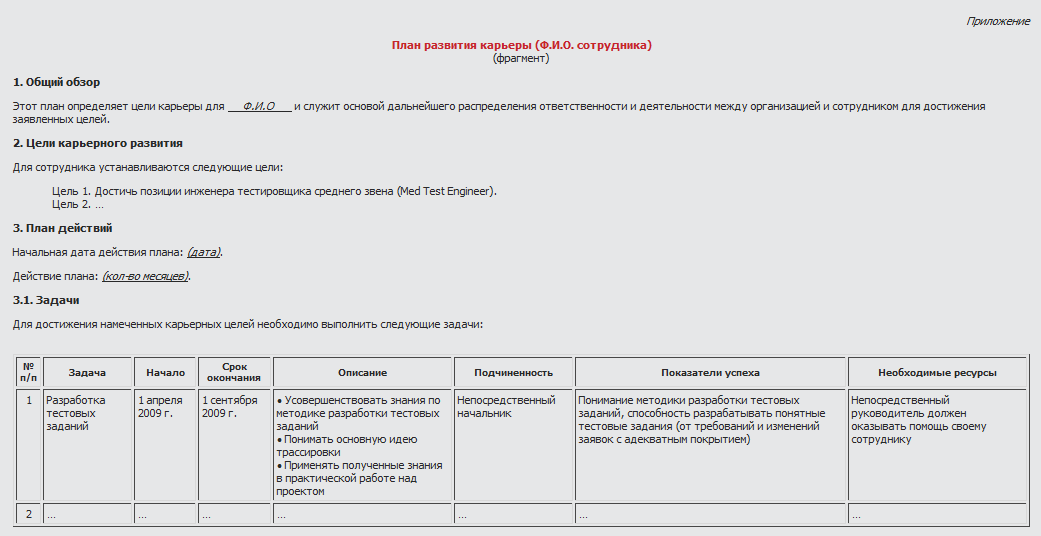
\includegraphics[height=0.73\textheight]{11-IT-specialist's-way/ipl.png}}
\end{frame}

\begin{frame} \frametitle{Пример индивидуального плана развития: заголовок и общий обзор }
 \begin{block}{ Заголовок}
План развития карьеры (ФИО сотрудника)
\end{block}
 \begin{block}{ Общий обзор}
Этот план определяет цели карьеры для (ФИО сотрудника) и служит основой дальнейшего распределения ответственности и деятельности между организацией 

и сотрудником для достижения заявленных целей
\end{block}
\end{frame}

\begin{frame} \frametitle{Пример индивидуального плана развития: цели карьерного развития и план действий }
 \begin{block}{ Цели карьерного развития}
Для сотрудника устанавливаются следующие цели:
\begin{itemize}
  \item Достичь позиции инженера тестировщика среднего звена
  \item ...
  \end{itemize}
\end{block}
 \begin{block}{ План действий}
Начальная дата действия плана: (дата)

Действие плана: (количество месяцев)
\end{block}
\end{frame}

\begin{frame} \frametitle{Пример индивидуального плана развития: задачи }

 \begin{block}{ Задачи}
Каждая задача представлена несколькими полями 

в таблице, а именно:
\begin{itemize}
  \item № задачи
  \item Задача
  \item Срок окончания
  \item Описание
  \item Подчиненность
  \item Показатели успеха
  \item Необходимые ресурсы
  \end{itemize}
\end{block}


\end{frame}

\begin{frame} \frametitle{Пример индивидуального плана развития: конкретная задача }

\begin{itemize}
  \item № задачи: 1
  \item Задача: Разработка тестовых заданий
 \item Начало: 1 апреля 2009 
  \item Срок окончания: 1 сентября 2009 
  \item Описание: \begin{enumerate}
 \item Усовершенствовать знания по методике разработки тестовых заданий
\item Понимать основную идею трассировки
\item Применять полученные знания в практической работе над проектом
  \end{enumerate}
  \item Подчиненность: Непосредственный начальник
  \item Показатели успеха: Понимание методики разработки тестовых заданий, способность разрабатывать понятные тестовые задания
  \item Необходимые ресурсы: Непосредственный руководитель должен оказывать помощь сотруднику
  \end{itemize}



\end{frame}

%\section{}
\lecturenotes

Текст конспекта, относящийся к слайду с указанием источника~\cite[с.~97--99]{Brooks}.

На интернет-источники можно ссылаться не по ГОСТу, но с обязательной гиперссылкой~\cite{Fowler}.

\begin{thebibliography}{99}
\bibitem{Sonmez} Сонмез Джон Путь программиста.Человек эпохи ИТ. СПб~: Питер, 2016.
\bibitem{mc} \href{https://dou.ua/lenta/columns/karta-kariery/?from=foo}{ Карта карьеры.}
\bibitem{itcf} \href{https://www.itcareerfinder.com/it-careers.html}{ IT Careers.}
\bibitem{hh} \href{https://hh.ru}{ Вакансии. }
\bibitem{rab} \href{https://www.rabotka.ru/job_description/}{ Должностные инструкции. }
\bibitem{JMSL} \href{http://www.dataart.ru/news/junior-middle-senior-lead-etc-v-chem-raznitsa/}{ Сергей Марков Junior, Middle, Senior, Lead.}
\bibitem{IPl} \href{http://www.e-reading.club/chapter.php/1050422/98/Beron_-_Upravlenie_rezultativnostyu.html}{ Составление индивидуального плана развития.}
\bibitem{IPlan} \href{http://www.sbsc.ru/books/TalentWarBook.pdf}{ Составление индивидуального плана развития.}
\end{thebibliography}

\end{document}

%%% Local Variables: 
%%% mode: TeX-pdf
%%% TeX-master: t
%%% End: 
